\documentclass[12pt,twoside,numbers=endperiod]{scrreprt}
\addtokomafont{disposition}{\rmfamily}
\usepackage[utf8]{inputenc}
\usepackage{graphicx}
\graphicspath{{images/}}
\usepackage{caption}
\usepackage{subcaption}
\usepackage[a4paper,width=150mm,top=25mm,bottom=25mm,bindingoffset=6mm]{geometry}
\usepackage{fancyhdr}
\usepackage{natbib}
\usepackage{parskip}
\usepackage{eurosym}
\usepackage{float}
\usepackage{url}
\usepackage{minted}
\usepackage{listings}
\usepackage{afterpage}
% \usepackage{ftnxtra}
% \usepackage{fnpos}
% \usepackage{titlesec}
\usepackage{setspace}
\usepackage{ltablex}
\usepackage{spverbatim}
\usepackage{makecell}
\usepackage[export]{adjustbox}
\usepackage{hyperref}
\usepackage{wrapfig}

% \renewcommand\chapterformat{\chapapp\ \thechapter}
\renewcommand\sectionformat{\thesection\hspace{1em}}
\renewcommand\subsectionformat{\thesubsection\hspace{1em}}

%%% START koma
\setkomafont{chapter}{\normalfont\bfseries\Huge}
\renewcommand\chaptername{}
\RedeclareSectionCommand[
  innerskip = 0pt,
  beforeskip = 0pt,
  afterskip = 10pt
]{chapter}
\RedeclareSectionCommands[
%   innerskip = 0pt,
  beforeskip = 5pt,
  afterskip = 2pt
]{section, subsection, subsubsection}
%%% END koma

%%% START titlesec
% \titleformat{\chapter}%
%   {\normalfont\bfseries\Huge}{\thechapter.}{10pt}{}
% \titlespacing*{\chapter}{0pt}{0pt}{10pt}
% \titlespacing*{\section}
% {0pt}{5ex}{2ex}
% \titlespacing*{\subsection}
% {0pt}{5ex}{2ex}
% \titlespacing*{\subsubsection}
% {0pt}{5ex}{2ex}
%%% END titlesec

\pagestyle{fancy}
\fancyhead{}
\fancyhead[CO,CE]{\nouppercase{\leftmark}}
\fancyfoot{}
\fancyfoot[CO,CE]{\thepage}
\lstset{
  breaklines=true,
  basicstyle=\ttfamily
}
\renewcommand{\chaptermark}[1]{%
\markboth{\thechapter.\ #1}{}}
\renewcommand{\baselinestretch}{1.2}
\renewcommand{\headrulewidth}{0.4pt}
\renewcommand{\footrulewidth}{0.4pt}
\newcommand{\npara}{
  \parskip=8pt
  \parindent=0.2in
}
\newcommand{\textbi}[1]{\textbf{\textit{#1}}}
\newcommand{\code}{\texttt}
    
\begin{document}

\definecolor{codeblock}{rgb}{0.86, 0.86, 0.86}

\begin{titlepage}
  \begin{center}
    \Large
    A thesis submitted for the Master of Science degree in Geospatial Technologies
    
    \vspace*{0.8cm}

    \Huge
    \textbf{Decentralised Location-Based Reputation Management System in IoT using Blockchain}

    \vspace*{1cm}

    \Large
    \textbf{Composed by Ponlawat Weerapanpisit}

    \vspace{1cm}

    \normalsize
    \centering\textbf{Supervised by Ph.D Sergio Trilles}

    \textbf{Co-supervised by Prof. Joaqu\'{i}n Huerta \& Prof. Marco Painho}

    \vspace*{2cm}

    
\includegraphics[scale=0.5]{images/uji.png}

    \vspace*{2cm}



    Universitat Jaume I

    \vspace*{0.8cm}

    05.03.2021

    \end{center}
\end{titlepage}

\pagenumbering{Roman} 

\thispagestyle{plain}
\begin{flushleft}
  \LARGE
  \textbf{Abstract}
  \vspace{0.4cm}
  \large
\end{flushleft} \label{Abstract}

\npara Internet of Things (\hyperref[Acronym-IoT]{IoT}) allows an object to connect to the internet network and observe or interact with a physical phenomenon.
The communication technologies allow an \hyperref[Acronym-IoT]{IoT} device to discover and communicate with another one to exchange services like humans do in their social network.
Knowing the reputation of another device is important to consider if it will trust before establishing a new connection to avoid an unexpected behaviour.
The reputation of a device can also be varied depending on its geographical location.
Thus, this thesis proposed an architecture to manage reputation values of end devices in an \hyperref[Acronym-IoT]{IoT} system, based on their located area.
To avoid a hard workload of the system in the cloud layer, the proposed architecture follows the cloud-fog-edge concept by adding an intermediate layer called a fog layer.
In this layer, multiple smaller devices are distributed, so it used the Blockchain technology to keep the reputation management to be consistent and fault-tolerant across different nodes in the layer.
Ethereum, which is a Blockchain implementation, was used in this work to ease the management functionalities, because it allows the Blockchain network to run a decentralised application through the Smart Contracts.
The location-based part of the system was done by storing geographical areas in the Smart Contracts, and make the reputation values to be subjected to different regions depending on device geographical location.
To reduce the spatial computation complexity in the Smart Contracts, the geographical data are geocoded by either one of two different spatial indexing techniques called Geohash and S2.
This work introduced three experiments to test the proposed architecture, to deploy the architecture in \hyperref[Acronym-IoT]{IoT} devices, and to compare the two geocoding techniques in the Smart Contracts.
It also additionally proposed a compression algorithm of the geocoded data.
The results showed that the proposed architecture is able to serve the objective of managing the reputation values based on location in a decentralised way.
The test case scenario also demonstrated that the \hyperref[Acronym-IoT]{IoT} devices were able to work as a Blockchain node.
They also were able to discover the service providers in an area and obtain their reputation values by querying through the fog layer.
Lastly, the comparison experiment results showed that Geohash performed better inside the developed Smart Contracts, while S2 encoded the data much faster outside the Smart Contracts.
The proposed compression algorithm of geocoded data resulted in a significant size reduction, but it was computationally heavier in the developed Smart Contracts.

\npara \textbf{Keywords:}
  \textit{Internet of Things (\hyperref[Acronym-IoT]{IoT})},
  \textit{Location-Based Trust and Reputation Management},
  \textit{Spatial Indexing},
  \textit{Ethereum Smart Contract},
  \textit{Decentralised Application}


% \chapter*{Dedication} \label{Dedication}
Lorem ipsum dolor sit amet, consectetur adipiscing elit, sed do eiusmod tempor incididunt ut labore et dolore magna aliqua. Ut enim ad minim veniam, quis nostrud exercitation ullamco laboris nisi ut aliquip ex ea commodo consequat. Duis aute irure dolor in reprehenderit in voluptate velit esse cillum dolore eu fugiat nulla pariatur. Excepteur sint occaecat cupidatat non proident, sunt in culpa qui officia deserunt mollit anim id est laborum.


\chapter*{Acknowledgements} \label{Acknowledgements}

\npara First of all, I would like to express my sincere thankful gratitude to Ph.D. Sergi Trilles, supervisor, for his helpful advice and feedback towards the whole work, from topic proposal stage until the conclusion.
Giving my special thanks to Prof. Joaquín Huerta and Prof. Marco Painho as well for being co-supervisor of this work.

\npara In addition, expressed here my thanks to the colleagues of this master programme in Geospatial Technologies, for all in Universitat Jaume I, Universität Münster, and Universidade NOVA de Lisboa, for sharing thoughts and knowledge during the course.

\npara Moreover, I convey my grateful to Erasmus Mundus programme for the scholarship as being financial support during this master programme.

\npara Lastly, I would like to express my thanks to my family for always being supportive despite the distance.


\setcounter{secnumdepth}{3}
\setcounter{tocdepth}{3}
\label{TableOfContents} \tableofcontents

\label{ListOfFigures} \listoffigures
% \addcontentsline{toc}{chapter}{List of Figures}

\label{ListOfTables} \listoftables
% \addcontentsline{toc}{chapter}{List of Tables}

\chapter*{Acronym} \label{Acronym}
\begin{tabular}{|l|l|}
  \hline
  \textbf{Abbreviation} & \textbf{Meaning} \\
  \hline
  \label{Acronym-ABI} ABI & Application Binary Interface \\
  \label{Acronym-API} API & Application Programming Interface \\
  \label{Acronym-CPU} CPU & Central Processing Unit \\
  \label{Acronym-ECDSA} ECDSA & Elliptic Curve Digital Signature Algorithm \\
  \label{Acronym-EVM} EVM & Ethereum Virtual Machine \\
  \label{Acronym-GIScience} GIScience & Geographic Information Science \\
  \label{Acronym-GPS} GPS & Global Positioning System \\
  \label{Acronym-GSM} GSM & Global System for Mobile Communications \\
  \label{Acronym-HTTP} HTTP & Hypertext Transfer Protocol \\
  \label{Acronym-HTTPS} HTTPS & Hypertext Transfer Protocol Secure \\
  \label{Acronym-IEEE} IEEE & Institute of Electrical and Electronics Engineers \\
  \label{Acronym-IoT} IoT & Internet of Things \\
  \label{Acronym-IP} IP & Internet Protocol \\
  \label{Acronym-JSON} JSON & JavaScript Object Notation \\
  \label{Acronym-LAN} LAN & Local Area Network \\
  \label{Acronym-LED} LED & Light Emitting Diode \\
  \label{Acronym-MQTT} MQTT & Message Queuing Telemetry Transport \\
  \label{Acronym-NPM} NPM & Node Package Manager \\
  \label{Acronym-OOP} OOP & Object-Oriented Programming \\
  \label{Acronym-RFID} RFID & Radio Frequency Identification \\
  \label{Acronym-SDN} SDN & Soft Defined Network \\
  \label{Acronym-SIoT} SIoT & Social Internet of Things \\
  \label{Acronym-SSH} SSH & Secure Shell \\
  \label{Acronym-WKB} WKB & Well-Known Binary \\
  \label{Acronym-UML} UML & Unified Modeling Language \\
  \label{Acronym-URL} URL & Uniform Resource Locator \\
  \label{Acronym-VPN} VPN & Virtual Private Network \\
  \hline
\end{tabular}

\newpage

\pagenumbering{arabic}

\chapter{Introduction} \label{Introduction}
\section{Context and Motivation} \label{Introduction-Context}

% Internet of Things
\npara \textbi{Internet of Things} or \hyperref[Acronym-IoT]{IoT} has recently played an important role in connecting physical objects into the internet network.
The development of hardware capabilities and communication technologies allow an object or a \textit{thing} in our daily lives which is equipped with sensors or actuators to connect to the internet network.
This process turns them into smart objects that can interact with users or with other devices in order to observe a physical phenomenon and perform an interaction \citep{SEnviro}.

% Trust in General
\npara In human society, there might be a number of service providers offering services that we need.
When a person wants to interact or consume the service from another, it is necessary to know how \textbi{trustworthy} they are, before one can decide to choose and start an interaction.
The way to know this trustworthiness can be based on the experienced users' recommendations, as well as from the evaluation based on service quality.
This is to guarantee that the service will satisfy users and will not cause consequent failures.

% Trust in IoT
\npara In the same way, an \hyperref[Acronym-IoT]{IoT} device can also communicate with each other in order to consume or provide services.
Figure \ref{fig:SIoTLuigiA} from \cite{SIoTSocialStructure}'s work shows a comparison between the components of social networks in humans and digital objects.
Trustworthiness management is a component that is relevant to the relationship management in human social networks.
To ensure that the provided services are reliable and not leading to consequent failures, it is important to consume the services from trusted providers.
Despite the fact that \textbi{trust} is a subjective concept and differs on each individual agent, it can be influenced by a quantity value such as \textbi{reputation index} which is a social quantity property of an agent \citep{ComputationalModelTrust}.
In consequence, it is necessary for an \hyperref[Acronym-IoT]{IoT} system to have an architecture that allows the management of device \textit{reputation indices} in the system, so that the devices that consume a service can use the value to decide whether they would trust the provider before establishing a new connection.

\begin{figure}[hbt!]
  \centering
  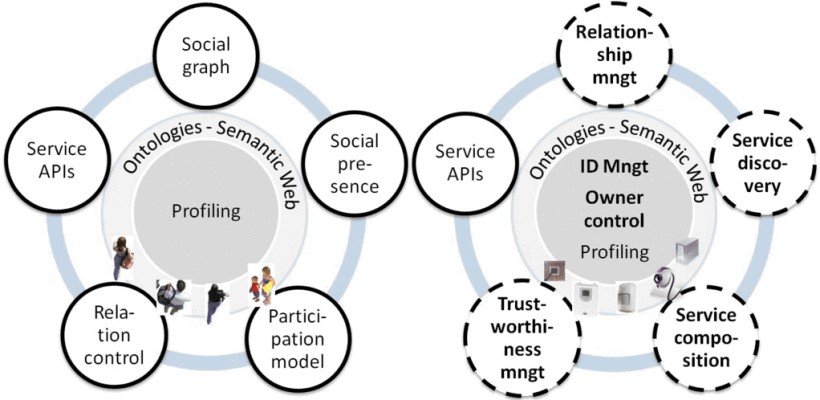
\includegraphics[width=\textwidth]{images/SIoTLuigiA.jpg}
  \caption{The components of social networks in human (left) and machines (right) \citep{SIoTSocialStructure}}
  \label{fig:SIoTLuigiA}
\end{figure}

% Area-based reputation
\npara Devices in an \hyperref[Acronym-IoT]{IoT} system are usually distributed over the geographical space and are able to move across different areas.
The location of the devices can be a factor that affects their trustworthiness \citep{TrustEnhancedSecurityLocationBased}.
For this reason, this master thesis will use this location component to build a reputation management system architecture to manage \hyperref[Acronym-IoT]{IoT} relationships.
In other words, it will include the spatial context of devices in order to establish the reputation values.

% Cloud-Fog-Edge architecture
\npara Another related technology is \textbi{cloud-fog-edge architecture}, which is a hierarchical architecture in the \hyperref[Acronym-IoT]{IoT}.
It divides the system into three layers which are \textit{cloud}, \textit{fog}, and \textit{edge} layer.
While the traditional cloud and edge layer were designed for heavy processing and low-level computation respectively, the fog layer was later proposed by Cisco to be an intermediate layer between these two layers \citep{CiscoUnleashFog}.
The capacity of a fog hardware is generally lower than the one in the cloud, but greater than edge devices enough so it can perform more complex calculations.
Hence, not all unnecessary computations have to be loaded in only cloud layer.
Moreover, the instalment of fog devices is also compromised in the extend between cloud and edge layers.
They are therefore generally geographically distributed, which are ideal to cover the location-based reputation management system.

% Blockchain
\npara The last related concept is \textbi{decentralisation}.
Due to the existence of fog layer, the intermediate devices are now distributed and not all computations need to be in the cloud layer.
\textbi{Blockchain} is a technology that allows data to be stored in a distributed way.
All nodes in a Blockchain network will share and possess the same data which are formed in blocks chronologically linked to each other like a chain.
The chain is distributed over the network which makes the system to be transparent and fault-tolerant \citep{BlockchainAdvantages}.
The Blockchain technology relies on hashing and consensus algorithms to confirm that all nodes in the network are having the same valid data, and it is not easy to tamper the chain.
The implementation of the Blockchain are well-known in \textbi{cryptocurrency}, such as Bitcoin and Ethereum.
But in the Ethereum, besides storing the money transactions it also allows \textbi{Smart Contract} which is an executable programme to be stored and callable from the Blockchain network.
In the other words, the Ethereum Blockchain network acts like a virtual machine that has the advantages of decentralisation in Blockchain.
Thus, this thesis proposes to adopt the Ethereum Smart Contract in the fog layer to create a decentralised application that is able to manage the reputation indices of an \hyperref[Acronym-IoT]{IoT} system.

\npara However, even the decentralised applications can execute any programming like a real computer does, but the characteristics of the Blockchain limit the ability of complex calculations in Smart Contracts.
Geometric spatial objects and their calculation which are related to complex algorithms and complicated data structures could cost an expensive computation in the Blockchain network.
For this reason, this thesis will use spatial indexing techniques in the implementation to study and challenge the possibility of manipulating spatial data in the Blockchain.
There are two hierarchical spatial indexing techniques being studied in this thesis.
The first one is \textbi{Geohash} which is an indexing technique invented by Gustavo Niemeyer \citep{GeohasUUID}.
And the second one is \textbi{S2} which was invented by Google engineers \footnote{\url{https://github.com/google/s2geometry}}.
Both techniques share the same hierarchical characteristics despite their different algorithms behind.
This thesis will therefore study the characteristics of these two techniques and compare their usage in the decentralised applications.

\section{Aims and Objectives} \label{Introduction-Aims}

\npara The main objective of this work is to propose a decentralised \hyperref[Acronym-IoT]{IoT} architecture which allows the location-based management of device services and their reputation values using Blockchain.

\npara To accomplish the main objective, this work will propose an \hyperref[Acronym-IoT]{IoT} architecture based on cloud-fog-edge structure, and decentralise the management system in the fog layer using the Ethereum Smart Contract.
Secondly, it will study and compare two spatial indexing techniques of Geohash and S2 which are used to represent the geographical data in the system, as well as implement and analyse their usage in the Smart Contracts.
Finally, it will simulate the architecture by implementing and deploying the system in the real \hyperref[Acronym-IoT]{IoT} devices.

\section{Research Questions} \label{Introduction-ResearchQuestions}

\begin{enumerate}
  \item \label{ResearchQuestion-DecentralisedFog} Is it possible to implement a decentralised area-based reputation management system of an IoT system in the fog layer using Blockchain?
  \item \label{ResearchQuestion-SpatialBlockchain} Is it possible to manipulate spatial data in a Blockchain network based on spatial indexing techniques?
  \item \label{ResearchQuestion-Geocoding} Comparing \textbi{Geohash} and \textbi{S2} geocoding techniques, which one does perform better in the proposed architecture, regarding speed, size, and suitability?
\end{enumerate}

\section{Document Structure} \label{Introduction-Structure}

\npara This thesis report is divided into five chapters.
The first chapter, \textbi{\nameref{Introduction}}, which is the current chapter, explains the motivation behind this work, the goals of the study, and the research questions.
Next chapter, \textbi{\nameref{Background}}, explains the related technologies and techniques.
There are three main topics related to this work, which are \textit{\nameref{Background-IoT}}, \textit{\nameref{Background-Blockchain}} and \textit{\nameref{Background-SpatialIndexing}}.
The third chapter, \textbi{\nameref{RelatedWorks}}, explores the literature of existing works that are related to the proposed architecture, as well as their technologies.
Fourthly, \textbi{\nameref{Methodology}}, explains the implementation design of this work.
It starts with the \textit{\nameref{Methodology-Architecture}} by introducing the whole picture of the proposed architecture, followed by the \textit{\nameref{Methodology-ExperimentDesign-Development}} which explains the tools and technologies used to develop the proposed architecture, and lastly, the \textit{\nameref{Methodology-ExperimentDesign}} elaborates the experimental procedures to test and evaluate the architecture.
After that, the fifth chapter of \textbi{\nameref{Results}} shows the development and experiment results of the architecture.
Followed by \textbi{\nameref{Conclusion}}, the last section which concludes the work and summarises experiment results, as well as suggests for the future development.
Finally, in the final part of the report, \textbi{\nameref{Appendix}} elaborates and explains related technologies and the data structures that could not be included in the previous chapters.


\chapter{Background} \label{Background}
\section{Internet of Things (IoT)} \label{Background-IoT}

% IoT
\npara The term \textbi{Internet of Things} or \textbi{\hyperref[Acronym-IoT]{IoT}} refers to the combination between network (internet), and physical objects (things).
It was firstly coined in 1999 by Kevin Ashton in his work of using \textit{Radio Frequency Identification} or \textit{\hyperref[Acronym-RFID]{RFID}} in a supply chain system \citep{ThatIoT}.
The \hyperref[Acronym-IoT]{IoT} devices rely on wireless communication technologies to connect them to the network.
Such technologies that allow the development of \hyperref[Acronym-IoT]{IoT} are for instance: Bluetooth, \hyperref[Acronym-RFID]{RFID}, Wi-Fi or \hyperref[Acronym-GSM]{GSM}.
As the technologies in wireless communication are continuously being developed and advanced, it allows IoT community to expand and grow significantly \citep{IoTVisionFuture}.

\subsection{Trust and Reputation System in IoT} \label{Background-IoT-Reputation}

% SIoT
\npara \textbi{Social Internet of Things} or \textbi{\hyperref[Acronym-SIoT]{SIoT}} is an integrated concept between \hyperref[Acronym-IoT]{IoT} and human social networking.
The idea is that the things in an \hyperref[Acronym-IoT]{IoT} system can discover the other devices which provide the needed services, establish a relationship and communicate with them \citep{SIoT}.
As humans do in their social life, when a person wants to know someone, or use a business service, they must know how reliable it is.
Also in the computer systems, when a device wants to use a service from the other devices, before establishing a connection with them, it should know whether the source is \textbi{trustworthy} in order to avoid problems or failures due to unexpected behaviours.

% Reputation and Trust
\npara The concept of \textbi{trust} is very subjective to each individual.
\cite{ComputationalModelTrust}'s study says that \textbi{trust} is a subjective expectation that one agent has toward another one.
It is used for expecting their future behaviours based on the encountered history.
\cite{SurveyOfTrustInComputerScience} divides the obtainment of trust in a computer system into two categories: policy-based trust and reputation-based trust.
A policy-based trust is centralised and the decision criteria are based on a third party.
The second one is based on \textbi{reputation}, which is a quantitative property derived by observed actions or behaviours in the past of one agent.
Hence, the non-centralised characteristic of the reputation-based trust allows an individual to subjectively decide its trustworthiness.

\subsection{Cloud-Fog-Edge Architecture} \label{Background-IoT-CloudFogEdge}

% Fog Introduction
\npara As the \hyperref[Acronym-IoT]{IoT} is growing and its related technologies are moving forward, an \hyperref[Acronym-IoT]{IoT} system could expand to a larger number of devices and connected sensors.
This raised consequent issues such as heavy processing and big data storage in the cloud layer or exceeding bandwidth in the network.
To tackle the problem, Cisco company proposed a solution by adding an intermediate layer between the cloud and end-device (edge) layers, called the \textbi{fog layer} \citep{CiscoUnleashFog}.

% Cloud-For-Edge
In a general \textbi{cloud-fog-edge architecture}, the \textbi{edge layer} is the most bottom layer where the end-devices are.
The devices in this layer are simplest and have less computation ability, connected to sensors or actuators in order to observe a physical phenomena or to have an interaction.
The end-devices are generally in a larger amount, and they should not perform any complex computation because they have limitations regarding hardware specification, memory and power consumption.

\npara Secondly, the \textbi{fog layer} is the intermediate layer.
The devices in this layer have more computation ability and can handle preliminary data processing as well as to store sensory data before forwarding them to the cloud layer.
In opposite direction, the fog layer can also be a middle party that passes commands or messages from the cloud layer to the edge layer.
Because the fog layer can also be geographically distributed, it can organise the edge devices in its responsible area.

\npara The last one is the \textbi{cloud layer}, which is the topmost layer in the architecture and is in charge of processing final data, managing the whole system, and storing the sensory data.
A cloud device is supposed to be physically static, and located in a data centre or a dedicated place.
The device itself can be either a dedicated server where the organisation administrator has responsibility of administration and maintenance.
Or it can be a cloud service in a form of platform-as-a-service (PaaS) or software-as-a-service (SaaS) which is provided by an external cloud service provider such as Microsoft Azure, Amazon Web Service (AWS), or Google Cloud.

%%

\section{Blockchain} \label{Background-Blockchain}

\npara \textbi{Blockchain} is a technology to store computer data in a distributed and decentralised way.
A Blockchain network is consisted of a number of \textbi{blocks}.
In a block there are \textbi{transactions} to store the data in the network.
Blocks and transactions are uniquely identified by using a cryptography hashing algorithm.
The identifier hashes of the blocks are used to link each other in a chronological linear sequence like a chain, which is the reason behind its name.

\subsection{Fundamental of Blockchain} \label{Background-Blockchain-Fundamental}

\npara \textbi{Blockchain} was originally mentioned by \cite{Bitcoin} (whose name is believed to be a pseudonym).
It proposed an electronic cash system that can store the transactions of ledgers in a decentralised way by using peer-to-peer communication.

\npara A Blockchain network has a number of blocks which are linked to each other in a chronological sequence.
As Blockchain was originally developed for storing money movements in an electronic currency called \textit{Bitcoin}, the data in each block are a set of money \textbi{transactions}.
A Blockchain node collects transactions from its clients and pack them into one block.
Then, the block is pushed to the end of the chain.
The node that has pushed the block will then broadcast the change to the other nodes in the same network to update the data.
Finally, the other nodes verify the change before updating their own chain.

\begin{figure}[htb!]
    \centering
    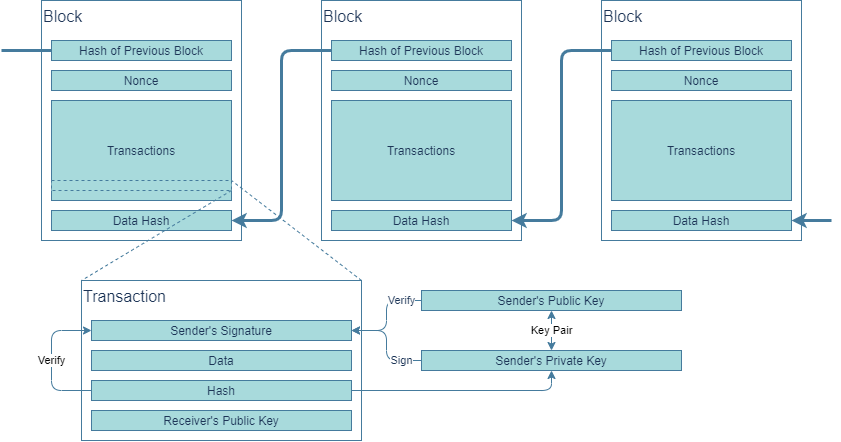
\includegraphics[width=\textwidth]{images/BackgroundBlockchain.png}
    \caption{Components of a block and transaction in a general Blockchain network}
    \label{fig:BackgroundBlockchain}
\end{figure}

\npara Figure \ref{fig:BackgroundBlockchain} shows the components inside a block.
One block contains:
  \textbi{hash of its previous block} which points to the last block in the chain before it was pushed,
  \textbi{nonce} which is a number to indicate the order of the block in the sequence,
  a set of \textbi{valid transactions},
  and the \textbi{hash} of the current block which will be referred when there is a new block afterwards.

\npara The validity of a transaction relies on the asymmetric key-pair cryptography.
A pair of \textbi{public key} and \textbi{private key} are both a set of binary data generated by mathematical techniques.
A public key can be published and generally used as an address or identifier of the owner.
In the other hand, a private key is supposed to be kept private.
It is used for signing the transaction to verify that the transaction is valid.
The public key can be generated by using a private key, but it is not possible to derive the private key from a public key.

\npara When a transaction has been generated, the creator uses its private key to sign the transaction using a mathematical calculation.
The result of the calculation is called \textbi{signature}.
The signature is then attached to the transaction before submitted to the block.
A signature can be verified whether it is valid or not by using the signer's public key.
In other words, a signature can be publicly verified by anyone but it can not be created without knowing the private key.
This is the reason why Blockchain can guarantee that the data inside will be secure and cannot be tampered even the data are visible and distributed across the network.

\npara The propagation of the data in a network becomes a problem when multiple peers want to push a new block at the same time, because the network should consider which chain from which peer node is valid and should be accepted in the chain.
This kind of problem is also known as Byzantine Generals Problem \citep{Byzantine}.
In Blockchain, the \textbi{consensus algorithm} is used to tackle the issue.
There are a number of different consensus algorithms that are used in different Blockchain implementations.
For example, Bitcoin and Ethereum uses \textbi{Proof of Work} consensus algorithm.
The Proof of Work gives a difficult mathematical challenge based on the \textit{nonce} value in the latest block.
The first node that can solve the problem has the right to push the block into the chain.
The process of calculating the mathematical problem is also called \textit{mining}.
The other examples of consensus algorithms are \textbi{Proof of Stake} which randomly select one node from the candidates using steak or wealth in the system as a random bias, or \textbi{Proof of Authority} which gives the right to an authorised node to add the block to the chain \citep{ConsensusAlgorithm}.

\subsection{Ethereum and Smart Contracts} \label{Background-Blockchain-Ethereum}

\npara \textbi{Ethereum} is a Blockchain implementation.
Similarly to Bitcoin, Ethereum blockchain also has its cryptocurrency called \textbi{Ether}.
The difference that makes Ethereum to be outstanding among developers is that Ethereum allows a block to store executable programmes.
This kind of applications is called \textbi{Smart Contract}.
A Smart Contract allows the execution and the storage of the programme stage to be done in a distributed and decentralised way.
The operation codes (opcode) in the Smart Contract were designed to be \textit{Turing complete}, which means that it can execute any programme algorithms that the actual computers can perform \citep{EthereumWhite}.

\npara Similar to the other Blockchain implementations, all nodes in Ethereum network contains the same transactions data, including Smart Contracts and their contract states.
This concept is like having a computer whose instances are distributed over the Blockchain network.
When a contract method is called, the node will add the method calling transaction into the chain.
The transaction can be interpreted and executed to update the contract state.
When the transaction is propagated over the network, the other nodes will also update their contract state in the same way.
This distributed machine is called \textbi{Ethereum Virtual Machine (\hyperref[Acronym-EVM]{EVM})}.

\begin{figure}[htb!]
  \centering
  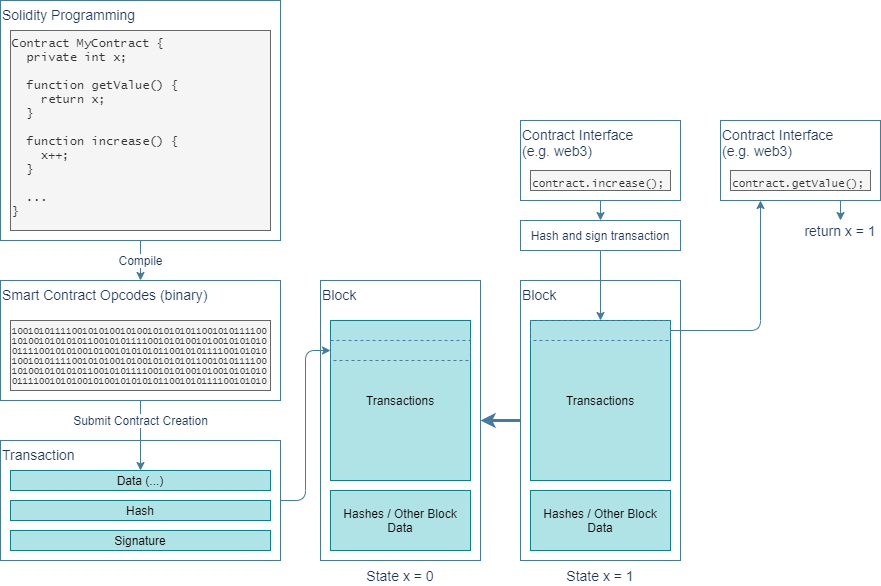
\includegraphics[width=\textwidth]{images/BackgroundEthereum.png}
  \caption{An example flow of contract creation and function calling in Ethereum Smart Contract}
  \label{fig:BackgroundEthereum}
\end{figure}

\npara Figure \ref{fig:BackgroundEthereum} shows the workflow of an Ethereum Smart Contract.
The top level programming language to write a Smart Contract can be either \textbi{Solidity} or \textbi{Vyper}, which has the similar syntax to JavaScript and Python respectively.
After that, the programming codes are compiled into Ethereum opcode binaries.
An opcode indicates a computational operation of the \hyperref[Acronym-EVM]{EVM} like an opcode in a computer programme.
These binaries data are then embedded into a transaction in a block and pushed into the chain.
The figure \ref{fig:BackgroundEthereum} also shows that calling method which changes the contract state (altering the variable value in the contract) needs to be submitted as another transaction in another block.
However, if the method is read-only (returns the contract state value without updating it), it can be called instantly without submitting as another transaction.

Calling a method in the Smart Contracts needs to be payed by its cryptocurrency.
The price of a method calling is determined by \textit{gas} spent in the calculation.
The concept of \textit{gas} is similar to the electric consumption in a physical computer.
Each opcode in a Smart Contract spends a different amount of gas determined by Ethereum\footnote{Ethereum gas per opcode: \hyperlink{https://docs.google.com/spreadsheets/d/1m89CVujrQe5LAFJ8-YAUCcNK950dUzMQPMJBxRtGCqs}{\code{https://docs.google.com/spreadsheets/d/\newline
1m89CVujrQe5LAFJ8-YAUCcNK950dUzMQPMJBxRtGCqs}}}.
The maximum amount of gas is limited by the Ethereum network.
For this reason, a method which has too many operations, especially iterations, is likely to cause an \textit{out of gas} error from the Ethereum network.

\npara

%%

\section{Spatial Indexing} \label{Background-SpatialIndexing}

\npara A computer processes and handles data in binary.
Therefore, the data that are not based on binary integer require more complicated data structures and different standards to work with, for instance, decimal (floating) number, text, picture, sound, as well as geospatial data.
Querying and accessing these types of data can be improved in performance and efficiency by using \textbi{indexing techniques}.
Indexing technique constructs the desired data to be a certain kind of search-able keywords.
When a user wants to query for the data, it can use a lookup table containing the sorted indices to quickly look for the position where the desired data are located.

\npara However, indexing the geographical data is more complicated as it is multidimensional and generally related to Euclidean space \citep{SpatialIndexing}.
There are different ways to index the geospatial data, for example, R-Tree which is based on a binary search tree for range query of destination spatial object \citep{RTrees}.
This thesis will focus on the geocoding-based indexing techniques to store and query for the spatial data objects in the Blockchain.

\npara \textbi{Geocoding} is the conversion of a geospatial object into another kind of interpretation.
Some geocoding techniques aim to ease human readability, postal address for example.
In the other hand, some of them aim to ease the readability and indexing in machine as the geocoded value is resulted in a binary integer, such as \textbi{Geohash} and \textbi{S2}, which are going to be studied in this thesis.
However, geocoding techniques are not two-way compatible.
In other words, the geocoded information cannot be reverted to the exact same geospatial object, but only to a similar one \citep{FastGeohash}.
Nevertheless, loss of accuracy is tolerable in this work, as its aim is not to store the exact geospatial data, but is to use them as an additional contextual information of the reputation management in an \hyperref[Acronym-IoT]{IoT} system.

\subsection{Geohash}

\npara \textbi{Geohash} is a hierarchical geocoding technique.
As it is hierarchical, Geohash representation does not have a fixed length, but the longer it is, the more precise geographical location it can describe.
A Geohash defines a location by storing binary bits of longitude in the odd positions, and latitude in the even positions (when the first position starts with 1).
However, it is more common to represent this group of binary bits into a textual representation, by grouping them into five bits per group and use \textbi{base32 representation} to textualise the data \citep{GeohashIndex}.
(Appendix \textit{\nameref{Appendix-Base32}})

\begin{figure}[htb!]
  \centering
  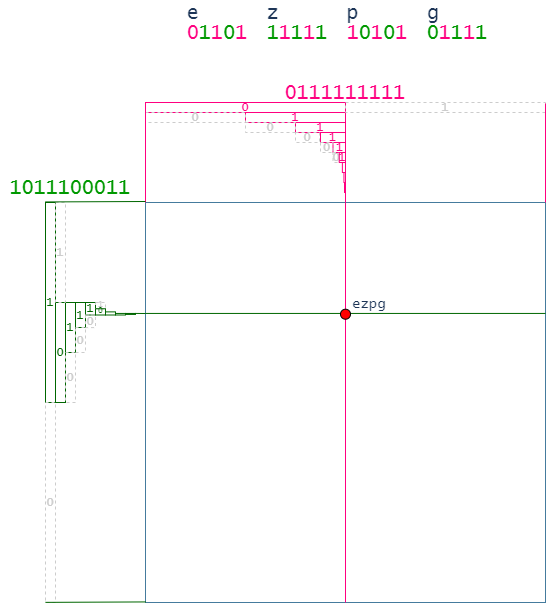
\includegraphics[width=\textwidth]{images/BackgroundGeohash.png}
  \caption{Example of the interpretation of a Geohash string into the geographical object}
  \label{fig:BackgroundGeohash}
\end{figure}

\npara Figure \ref{fig:BackgroundGeohash} shows an example of how Geohash works.
The figure gives an example of Geohash string \code{ezpg}.
The alphabets are base32-encoded character which can be converted to binary: \code{e} is \code{01101}, \code{z} is \code{11111}, \code{p} is \code{10101}, and \code{g} is \code{01111}.
Then, these binaries are concatenated.
Those bits at the odd positions (pink in Figure \ref{fig:BackgroundGeohash}) represent the longitude or x axis, and those at the even positions (green in Figure \ref{fig:BackgroundGeohash}) represent the latitude or y axis.
In the longitudinal bits, \code{0} represents the left side and \code{1} represents the right side.
But when the interpretation is on the geometric earth, it will start by taking the longitude 0° as the middle point.
When the bit is \code{0} it will travel to the minus side of the middle point (-180° to 0°), while in the case of \code{1} it will travel to the plus side of the middle point (0° to 180°).
For the next bit position, the new middle point will be calculated, and takes the same step over and over until the end of the sequence.
Similarly for the latitudinal bits, \code{0} represents the lower side from the middle point and \code{1} represents the upper side, when the first middle point is the equator.

\npara The Geohash then preserves the hierarchical property, as when it is represented by a less number of bits, the area (or the error) will be larger and is more difficult to define a point in the area.
But the more bits it gains, the smaller the area shrinks.
For this reason, two Geohashes having a mutual prefix means that they are located in the same cell at the upper level.

\subsection{S2}

\npara \textbi{S2} is another hierarchical geocoding technique similar to Geohash.
It is represented by an integer with a maximum of 64 bits in length.
Because it is hierarchical, like Geohash, the length of the representation can be reduced, but there will be a loss of its accuracy as the represented area will be bigger \citep{GeofencesBlockchain}.

\begin{figure}[htb!]
    \centering
    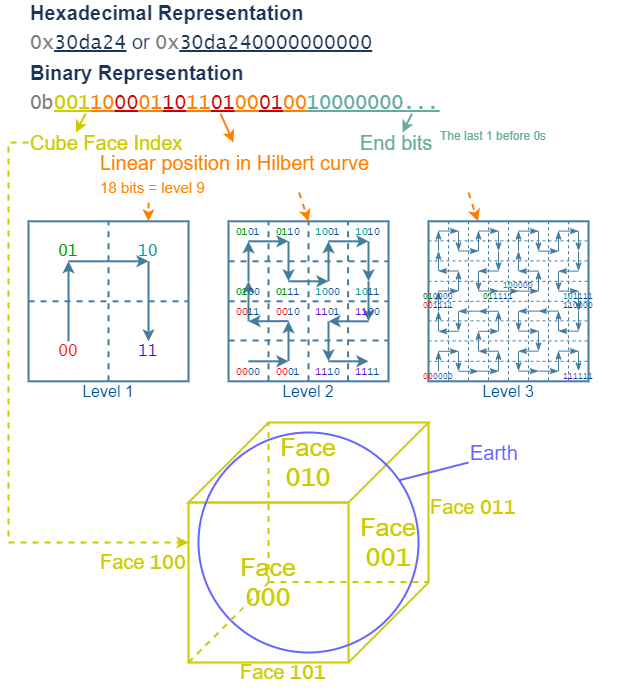
\includegraphics[width=\textwidth]{images/BackgroundS2.png}
    \caption{Example of interpretation of S2 cells}
    \label{fig:BackgroundS2}
\end{figure}

\npara One difference between Geohash and S2 is that S2 cells are based on the Hilbert space-filling curve, which is a line that travels through all the cells in a tabular space without making any loops.

\npara Figure \ref{fig:BackgroundS2} shows the characteristics and the interpretation of S2.
The length of an S2 representation can be 64 bits in maximum, but it can be trimmed to the desired level to reduce space consumption.
The end of S2 is determined by the last bit \code{1} that is followed by \code{0}s until the end of the data length.
Those bits before that are significant for calculation and cannot be cut, otherwise, the precision will be lost.
An area represented in S2 is called \textbi{cell}, which is the term that will be used in this thesis to refer a geocoded area in either Geohash or S2.

\npara As S2 uses a cube to fit the earth sphere and project the location to each face of the cube, the first 3 bits of an S2 cell are preserved for determining in which face the cell is falling in\footnote{\url{https://s2geometry.io/resources/earthcube}} (from \code{000} for the first face, until \code{101} for the sixth face).
The next set of the binary data represents the linear position on the Hilbert curve.
One cell position in the Hilbert curve contains 4 cells in the next level.
Hence, every level increment requires 2 more bits.

\npara The example in Figure \ref{fig:BackgroundS2} shows that \code{100001101101000100} contains 18 bits, which means the cell is located in 138,053\textsuperscript{rd} region in level-9 of the Hilbert curve, out of all 262,144 regions (which is 4\textsuperscript{9}).
The figure also demonstrates that, decreasing level of the Hilbert curve, the cell still covers the same region but in a bigger area.
This also implies that when two cells have a mutual prefix, they are located in the same cell of the upper level, which is the same property that Geohash also has.


\chapter{Related Works} \label{RelatedWorks}
\npara Decentralisation of the reputation management system in an \hyperref[Acronym-IoT]{IoT} system based on agent geographical locations is a relative new topic.
For this reason, there are no many direct related works.
This section divides the reviews of the literature into different related categories, which are \textit{\nameref{RelatedWorks-ReputationManagementSystem}}, \textit{\nameref{RelatedWorks-BlockchainIoT}}, and \textit{\nameref{RelatedWorks-Spatial}}.

\section{Trust and Reputation Management System} \label{RelatedWorks-ReputationManagementSystem}

\npara There are several related works regarding an IoT system architecture to manage reputation values and trusts.
In \cite{TrustArchitectureReputationEvaluation}'s work, the architecture divides the reputation management into five layers: reputation management layer, organisation layer, \hyperref[Acronym-SDN]{SDN} control layer, node layer and object layer.
Users requests for an operation of the \hyperref[Acronym-IoT]{IoT} device through the organisation layer, which is the middle way between the reputation management centre and the end nodes.
The organisation layer decides whether the requested node is trustworthy before executing the action.
Devices in this work do not execute their actions by themselves without a decision from the organisation layer.
\cite{TrustBasedAirQualitySensing} also purposed an interesting scenario of moving \hyperref[Acronym-IoT]{IoT} devices and an architecture to manage their trust values.
The work is based on a scenario of sharing air quality data, whose trust are evaluated by user's experience towards another target user in a different area.
The consumer chooses the most trustworthy data provider and decide whether the air quality in the target area is satisfying, so that they can move into the area.
The work is not based on the reputation value, which is a common expectation value towards one agent in the system, but it is based on a subjective trust, which is a one-to-one relationship between each device.
Furthermore, the management system is centralised in the cloud as all trust values of each device relationship are stored there, therefore the dependency of calculation and storage of the values are depend on the cloud layer.

\npara There were also works that tried to decentralise the trust management system as well.
\cite{PublicFogReputationEthereum}'s work proposed an architecture of a decentralised reputation management system in an Ethereum network by using Smart Contract.
In this work, end devices are in charge of evaluating the fog devices and store their reputation values in the Smart Contract.
The work is a good example of designing an architecture of reputation management using Smart Contract in \hyperref[Acronym-IoT]{IoT}.
However, the reputation value in this work is subjected to fog devices, not to edge devices, which serves different propose from this thesis.
Additionally, \cite{IoETrustBlockchain} has proposed a cloud-fog-edge-based architecture to manage trust values of devices in the system.
The Blockchain network is implemented in the fog layer.
In this architecture, an end device generates the reputation information of another device in a transaction, and sign it before submitting to the Blockchain network.
The values are stored in the Blockchain and, therefore, they are shared across different fog nodes in different areas.
However, the reputation value itself is the same even the device has moved to a different region.
A spatial context is not considered for managing the reputation values.

\section{Blockchain and IoT} \label{RelatedWorks-BlockchainIoT}

\npara In the previous section (\textit{\nameref{RelatedWorks-ReputationManagementSystem}}), there have been already mentioned some works using blockchain to serve trust management purpose:
  \cite{PublicFogReputationEthereum}'s uses Smart Contract in Ethereum to store reputation values of fog devices,
  and \cite{IoETrustBlockchain} uses Blockchain in fog layer to store reputation of devices.
This section explores more of the Blockchain usage in \hyperref[Acronym-IoT]{IoT} systems regardless of relevance to trust management system.

\npara \cite{ManageIoTBlockchain} implemented the Ethereum Smart Contract in an \hyperref[Acronym-IoT]{IoT} system to manage devices and control their behaviour policies.
The work shows that using of Smart Contract allows the system to configure device rules and able to control them in a distributed way.
\cite{RaspberryPiEthereum}'s work also showed the possibility of deploying Blockchain network in IoT devices by using Raspberry Pi as a node.
This implies that \hyperref[Acronym-IoT]{IoT} devices, comparing to modern computer, smaller in size, better in mobility, are powerful enough to run necessary computations for being a Blockchain node.

\section{Spatial Indexing} \label{RelatedWorks-Spatial}

\npara In the fundamental level, computer recognises all the digital data as binary integers, which means more complex data requires these binaries to be formed in a more complicated structure and have proper algorithms to work with them.
This applies to the geospatial data.
Digitalised lines, points or polygons in a space require binary representation.
It also needs indexing for speeding up the query.
This section explores the works that use spatial indexing techniques and their usage in Blockchain.

\npara \cite{SpatioTemporalComparison} compared different techniques of geocoding between raw geographical object (coordinates), Z-Order space-filling curve (Geohash), and Hilbert space-filling curve, in terms of computation, efficiency, and utility.
The study showed that geocoding using the Hilbert curve performed better in most of the aspects.
\cite{GeofencesBlockchain} used Geohash and S2 to fit a desired region.
The resulted cells were used for being a geofence, stored in a Smart Contract.
The work demonstrated the feasibility of handling spatial data in Smart Contracts.
They finally concluded that in their work S2 has a better performance than Geohash.


\chapter{Methodology} \label{Methodology}
\npara This chapter is divided into three main sections. Firstly, \textbi{\nameref{Methodology-Architecture}} proposes the architecture overview and its component in the system.
Secondly, \textbf{\nameref{Methodology-ExperimentDesign-Development}} describes tools and languages used for developing the proposed architecture.
The last part of this chapter, \textbi{\nameref{Methodology-ExperimentDesign}} elaborates how the experimental procedures will be held and how to evaluate the results.

\section{System Architecture} \label{Methodology-Architecture}

\subsection{Overall Architecture} \label{Methodology-Architecture-Overall}

\npara In this work, the reputation management system of \hyperref[Acronym-IoT]{IoT} devices is based on cloud-fog-edge architecture.
Each device in the fog layer is a node in the Ethereum Blockchain network.
In practice, the Ethereum network can be either public or private network.
However, in this work we encourage the private one because the management system is aimed to be decentralised in an \hyperref[Acronym-IoT]{IoT} system, not to be a public access for anybody.
The Smart Contracts deployed in the fog layer can store and manipulate edge devices, their services information, and geographical data of the associated regions.

\begin{figure}[hbt!]
  \centering
  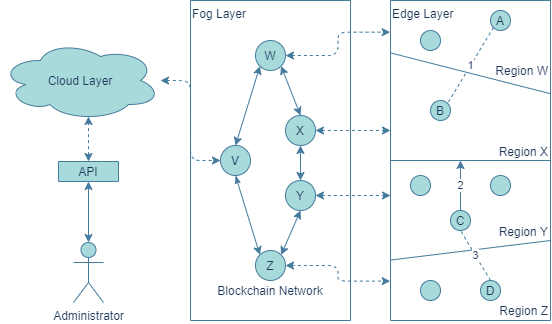
\includegraphics[width=\textwidth]{images/OverallArchitecture.png}
  \caption{Overall architecture of the proposed reputation management system}
  \label{fig:OverallArchitecture}
\end{figure}

\subsubsection*{Cloud layer}
\npara Cloud layer is generally in charge of storing and analysing data from edge sensors, as well as controlling, visualising and interacting with users.
However, in this work, because the management system is expected to be implemented in the fog layer, and the sensory data manipulation is not a protagonist in this thesis, so there will be less mentioning about this layer.
In a practical implementation of the proposed architecture, cloud layer can serve an \hyperref[Acronym-API]{API} for system administrators to control fog nodes in the layer.

\subsubsection*{Fog layer}
\npara Fog layer contains a number of devices which can be either geographically distributed or not.
These fog devices connect to each other and form an Ethereum Blockchain network \textit{to serve the Smart Contracts} for managing reputation indices and \textit{to serve the \hyperref[Acronym-API]{API}s} to interact with the contracts.
One fog device can be associated to a single or multiple regions.
However, it is not necessary because a fog device can be a Blockchain node without being associated to any regions.
For example from Figure \ref{fig:OverallArchitecture}, fog \textit{V} is not associated to any region, while fog \textit{W}, \textit{X}, \textit{Y}, \textit{Z} are associated to the region \textit{W}, \textit{X}, \textit{Y}, \textit{Z} respectively.

\subsubsection*{Edge layer}
\npara A device in this layer is equipped with sensors or actuators, and are designed to communicate with other devices in order to consume the services (dashed-line 1 from Figure \ref{fig:OverallArchitecture}).
The service consumption between devices will be based on their \textbi{trust}, which they can decide whether to trust a service provider by using the \textbi{reputation index} stored in the Smart Contracts from the fog layer.
Therefore, an edge device need to communicate with the fog layer to discover other devices in the area that provide needed services, and to query the reputation data of those providers.

\npara Furthermore, devices in the proposed system are assumed to be movable and can be displaced across the different areas.
Hence, when a device entered another area it should have a different reputation value because it is not recognised in the region.
For example, from Figure \ref{fig:OverallArchitecture}, device \textit{C} can move from region \textit{Y} to \textit{X} (arrow 2), but once it has moved, device \textit{D} which is its consumer should not anymore recognise its reputation.
And to consume the service it should establish a new connection with another device in the area that it can secondly trust.

\subsection{Scenario and Interaction Flows} \label{Methodology-Architecture-Flows}

\npara To achieve the architecture in Figure \ref{fig:OverallArchitecture} from the last section (\ref{Methodology-Architecture-Overall}).
This section elaborates the usage context of the architecture by designing interaction flows between each role in the system.
These flows will help to understand the functionalities of different components in the system, which are important for development design of programming classes and functions in the implementation section.

\npara The location-based reputation management system plays a role in the \hyperref[Acronym-IoT]{IoT} system when an end device has moved, or has requested to establish a connection with another device.
Therefore, this section divides the related interaction flows into three categories, which are 1) \textit{region management flow} which happens when there is a fog layer wants to associate itself to a geographical region in the system, 2) \textit{edge device mobility flow} which happens when an edge device has moved within the same or between different regions, and 3) \textit{reputation management flow} which happens when an edge device wants to consume a service from another device.

\begin{figure}[htb!]
  \centering
  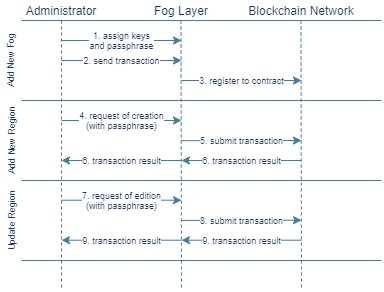
\includegraphics[width=0.8\textwidth]{images/WorkflowManageRegion.png}
  \caption{The workflow of region management in the system}
  \label{fig:WorkflowManageRegion}
\end{figure}

\npara Firstly, Figure \ref{fig:WorkflowManageRegion} shows the interaction when a fog node needs to assign or modify itself with a geographical area.
First of all, if the fog node is a new Blockchain node in the network, it needs to be assigned to an Ethereum address with a private key from the administrator (arrow 1).
After the device has been assigned to a unique Ethereum address, it can now interact with the Blockchain network.
Then, the administrator will send a contract transaction to register the node (arrow 2, 3).
After the node has been registered, it can now associate itself to a region to record that the region is in its responsibility.
The same flow happens when the node wants to update its region data.
To do so, the administrator calls a request of addition or edition to the fog node (arrow 4, 7), the node then interact with the Blockchain network to handle the request (arrow 5, 8).

\begin{figure}[htb!]
  \centering
  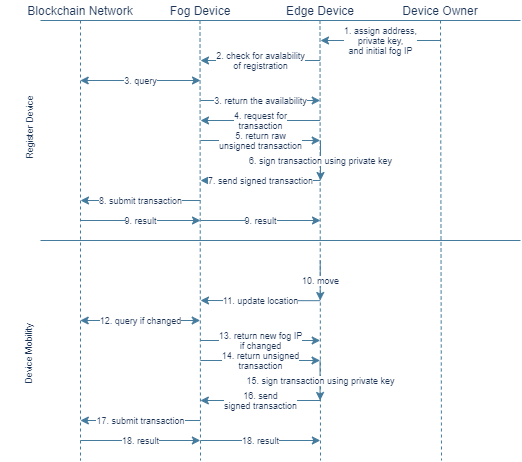
\includegraphics[width=\textwidth]{images/WorkflowMobility.png}
  \caption{The workflow of edge device mobility}
  \label{fig:WorkflowMobility}
\end{figure}

\npara Secondly, since the reputation values stored in the system are based on the device locations, it is necessary to consider the consequence when an end device has updated its location.
Figure \ref{fig:WorkflowMobility} shows the flow of the action.
As same as the fog layer, a device in the edge layer also needs its own identity in the Blockchain network so that it can interact with the Smart Contracts.
Hence, it is necessary to register a device to the Smart Contracts when it has been added to the system.
To do so, the device owner must assign a unique Ethereum address and its private key to the device (arrow 1).
Then, the device sends a contract transaction for registering.
However, due to the hardware limitations of those devices in the edge layer, it will be too big for them to store the contracts interface and be a Blockchain node.
For this reason, the interaction between the edge devices and the Smart Contracts will be done through the fog layer.
After the fog layer receives a \textit{registration request} from an edge device (arrow 4), it generates a \textit{raw unsigned transaction} and gives it back to the device (arrow 5).
The fog layer cannot sign the transaction for the edge device because it does not know the private key.
The edge device signs the transaction (arrow 6) and send the signature back to fog layer (arrow 7).
The fog layer submits the transaction to the Blockchain network (arrow 8).

\npara After the edge device has been registered, it can be referred in the Smart Contracts by using its Ethereum address.
Then, when the device has moved, it sends the updated location to the fog layer to check for the update if needed (arrow 11, Figure \ref{fig:WorkflowMobility}).
The fog layer checks with the Smart Contract whether it is necessary to update the device location data (arrow 12), in case of yes, it returns an unsigned transaction back to the device (arrow 14).
The device signs the transaction and return the signature to the fog layer (arrow 15, 16).

\begin{figure}[htb!]
  \centering
  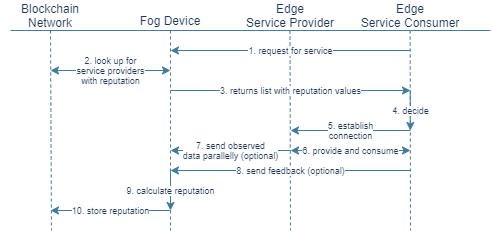
\includegraphics[width=\textwidth]{images/WorkflowReputation.png}
  \caption{The workflow of reputation query and generation}
  \label{fig:WorkflowReputation}
\end{figure}

\npara The last event is when a device wants to consume a service.
Figure \ref{fig:WorkflowReputation} shows the flow of this interaction.
The consumer requests for a service to the fog layer.
The fog node handles it by looking up for the results in the Smart Contracts (arrow 1, 2).
Then, it returns a list of candidate service providers and their reputation values in the area back to the consumer (arrow 3).
The consumer considers from this list and establish a new connection with the provider which it trusts the most (arrow 4, 5).
While the connection is ongoing (arrow 6), the service provider can parallelly sends the data to the fog device (arrow 7), which can later use these data to calculate the service quality as a factor of generating a new reputation index.
After the connection is finished, the consumer can send its feedback regarding the service to the fog node (arrow 8).
The fog layer finally have both sensory data from the provider and a feedback from the consumer, it then can use these information to calculate a new reputation index of the service provider (arrow 9) and update the value in the Smart Contracts (arrow 10).

\subsection{Fog Layer} \label{Methodology-Architecture-RMS-Fog}

\npara In the fog layer, there are two sub-components: \textbi{Ethereum Blockchain Network} which stores Smart Contracts of managing device information and the reputation data.
The second sub-component is \textbi{Fog \hyperref[Acronym-API]{API}} which is an \hyperref[Acronym-HTTP]{HTTP} interface for communication with the administrator users and edge devices.

\subsubsection{Ethereum Smart Contracts}

\begin{figure}[htb!]
  \centering
  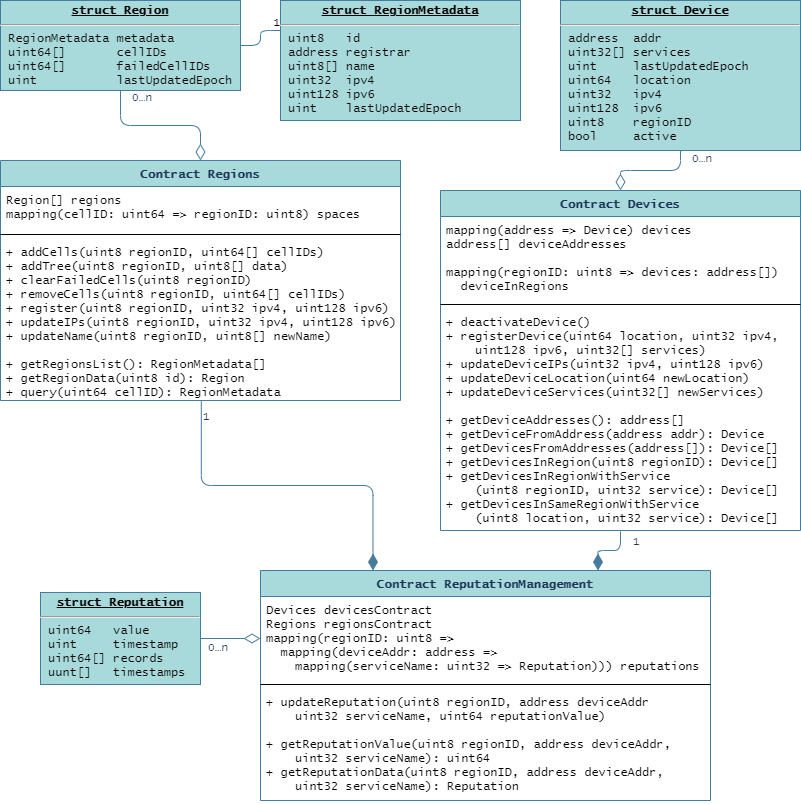
\includegraphics[width=\textwidth]{images/Contracts.png}
  \caption{Class diagram of the Smart Contracts}
  \label{fig:ContractsDiagram}
\end{figure}

A Smart Contract in the Ethereum Blockchain network can be written in \textit{Solidity} programming language.
The syntax of Solidity allows an object-oriented way of programming.
Hence, the structure of a Smart Contract can be described using a diagram similar to programming in other \hyperref[Acronym-OOP]{OOP} languages such as C\verb|#| or Java.
Nevertheless, the computation is slightly different comparing to a traditional programming language as there are some points needed to concern when doing Smart Contracts programming, such as:

\begin{itemize}
  \item Methods in Solidity can return more than one values.
  \item Decimal number: float or double, is not fully supported in Solidity \citep{SolidityTypes}, so integer or big integer is more encouraged.
  \item Similarly, strings are also not fully supported in Solidity.
  For this reason, manipulating and storing textual data should be done in binary level.
  \item When sending a contract method transaction, the Smart Contract always knows who is the transaction sender.
  Therefore, it is not necessary to define a caller in the method parameters.
\end{itemize}

\npara Figure \ref{fig:ContractsDiagram} shows the Smart Contract diagram of the proposed architecture.
There are three contracts in this proposed architecture:
  \textbi{Regions Contract} which manages the regions and their geospatial areas,
  \textbi{Devices Contract} which manages devices in the system and their service information,
  and finally \textbi{Reputation Management Contract} which enables updating and querying the reputation value in different regions.
In practice, each contract will have only one instance.
The regions and devices contract can be initiated and have an instance by their own.
In contradiction, the reputation management contract is dependent on the regions and devices contract in order to be functional.

\subsubsection{Fog API}

\npara Fog \hyperref[Acronym-API]{API} is another component inside a fog device which connects users to the Smart Contracts.
A user of this \hyperref[Acronym-API]{API} can be either the administrator who manages the system, or the edge devices that communicate for discovering service providers and their reputation values in an area.
The \hyperref[Acronym-API]{API} serves on \hyperref[Acronym-HTTP]{HTTP} protocol accepting the requests and returning responses in a \hyperref[Acronym-JSON]{JSON} format.
It communicates with the Ethereum client to serve the requests.
It also performs a preliminary condition checking before calling the Smart Contract to avoid an unexpected failure transaction.

\begin{figure}[ht]
  \centering
  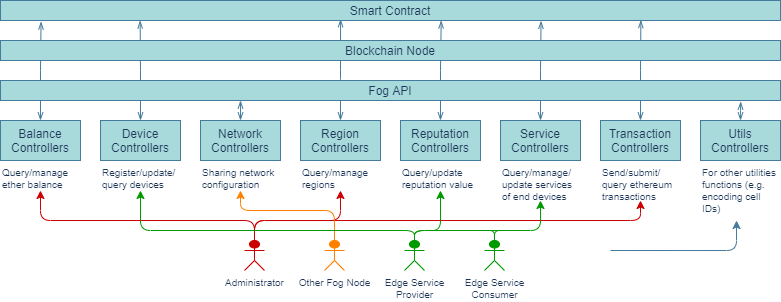
\includegraphics[width=\textwidth]{images/FogAPIs.png}
  \caption{Controllers and interaction diagram of Fog \hyperref[Acronym-API]{API}}
  \label{fig:FogAPIs}
\end{figure}

\npara The interaction interface of the Fog \hyperref[Acronym-API]{API} is divided into a number of different controllers which are listed in Figure \ref{fig:FogAPIs}.
Each controller serves a different propose and interact with different users in the system.
Most of the controllers require a connection to the Blockchain in order to query or submit a Smart Contract transaction, while some controllers are designed for the other facility and calculation proposes so they do not require any communication with the Ethereum client.

\subsection{Edge Layer} \label{Methdology-Architecture-RMS-Edge}

\npara The communication of edge devices in this work are also based on \hyperref[Acronym-API]{API} over \hyperref[Acronym-HTTP]{HTTP} protocol.
The device exposes its \hyperref[Acronym-IP]{IP} address and serves its \hyperref[Acronym-API]{API} in a defined port, so that a service consumer can communicate to consume the service.
Despite the fact that \hyperref[Acronym-HTTP]{HTTP} is used in the development of this work, it is not obligatory that another implementation adopting the architecture has to use the same communication technology.
The system architecture allows another technology as well, depending on their requirements and hardware specifications, \hyperref[Acronym-MQTT]{MQTT} for instance.
Nevertheless, to accomplish the proposed interaction flow, a device in this layer should be able to perform the calculation of signing a transaction using \textit{Elliptic Curve Digital Signature Algorithm (\hyperref[Acronym-ECDSA]{ECDSA})} which is a digital signature algorithm used in the Ethereum network.

\subsection{Geographical Data in the Smart Contract} \label{Methodology-SpatialSmartContract}

\begin{figure}[htb!]
    \centering
    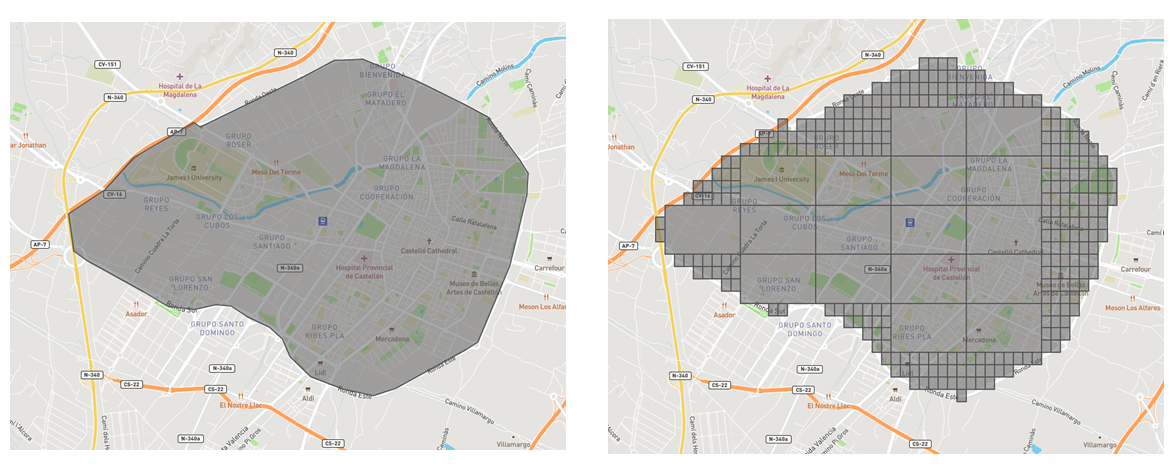
\includegraphics[width=\textwidth]{images/PolygonAndGeohashes.png}
    \caption{Example of a polygon covered by geocoded cells}
    \label{fig:PolygonAndGeohashes}
\end{figure}

\npara As described in the previous sections (\ref{Background-SpatialIndexing}, \ref{Methodology-Architecture-RMS-Fog}), this thesis decided to use geocoding techniques to store the geographical areas (polygons) of the associated regions in the Smart Contracts to manage the reputation and perform a spatial query.
Figure \ref{fig:PolygonAndGeohashes} shows an example of the geocoded regions.
The left image shows the original polygon of the region.
The data stored in the Smart Contract will be a set of geocoded cells shown in the right image.
Because of that the binary representation of the adopted geocoding techniques is hierarchical, it can merge the group of cells which fulfil the lower level into one cell in the upper level.
This behaviour can be observed from the right image of Figure \ref{fig:PolygonAndGeohashes}.
The cells in the centre of the region are merged into one bigger cell.

\begin{figure}[htb!]
  \centering
  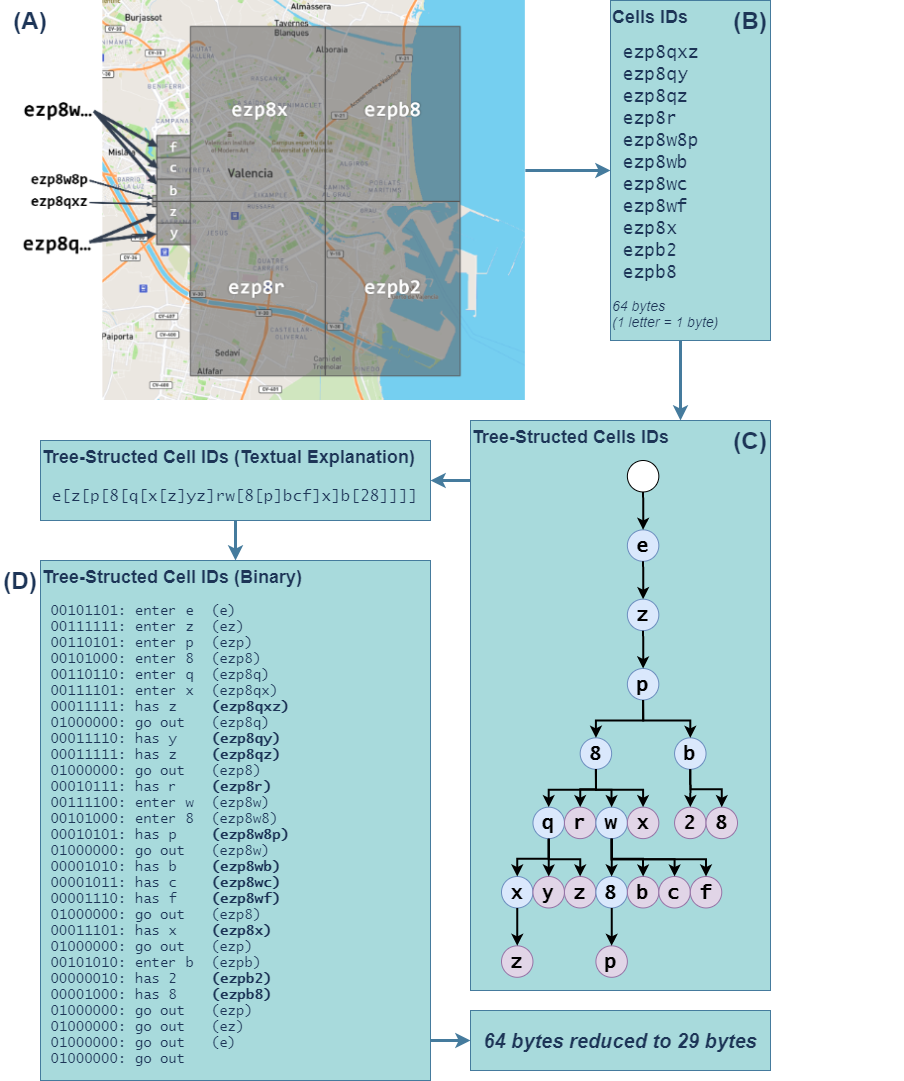
\includegraphics[width=\textwidth]{images/GeocodingCompression.png}
  \caption{An example of the proposed geocoded cells compression technique}
  \label{fig:GeocodingCompression}
\end{figure}

\npara Figure \ref{fig:GeocodingCompression} shows another example of geocoding a region.
Part \textit{(A)} of the figure shows the geocoded region cells and their identification using Geohash.
There are 11 cells from 3 different levels in this example.
Part \textit{(B)} of the figure shows the cell identification list of the region.
When a letter consumes 1 byte in the memory, this list of Geohash cells will consume at least 64 bytes of data, excluding cell separation such as a new-line character.
From this list it can be observed that there are redundancy of the data, especially the prefix of those cells.
Therefore, this work will also propose a compression technique of geocoded cells based on tree structure.
Part \textit{(C)} of Figure \ref{fig:GeocodingCompression} shows the tree-based structure of this geocoded region.
The nodes in blue colour represent the cells that have children, while the nodes in purple colour represent the final level that will be included in the region data.
This tree structure can be encoded into binary representation shown in part \textit{(D)} of the figure.
Because a Geohash cell uses \hyperref[Appendix-Base32]{\textit{base32}} representation, which requires only 5 bits to store one level, storing it in one byte will have 3 bits remained unused.
Therefore, these 3 bits can store an additional information to indicate that the node cell has children or not.
The result from binary encoding this tree requires only 29 bytes to store the data, which is less than a half of the original data that requires 64 bytes.

\npara In the same way, an S2 cell list can also be compressed by the same algorithm.
However, an S2 cell uses 2 bits for one level, storing one level of 2-bit in one byte is not sufficient.
Therefore, the S2 cell will be grouped by 6 bits before being structured to be a tree, the spare 2 bits are used for the level open or close marking like Geohash.
A 6-bit in this S2 cell can be represented by \hyperref[Appendix-Base32]{\textit{base64}} representation.

The description of compressed data is explained in the appendix (\textit{\nameref{Appendix-GeocodingCompress}}).

%%

\section{Implementation and Development} \label{Methodology-ExperimentDesign-Development}

\npara The proposed architecture is an abstract structure and can be implemented using any programming languages and tools.
However, this section will explain the tools used for developing the proof of the architecture in this thesis.

\subsection{Fog Layer}
\npara The Ethereum network will be deployed using \textbi{Go Ethereum (Geth)}\footnote{\url{https://geth.ethereum.org/}}, which is an open-sourced implementation of the Ethereum Blockchain network using Go language.

\npara The fog \hyperref[Acronym-API]{API} will be developed by \textbi{JavaScript} language run in \textbi{NodeJS}\footnote{\url{https://nodejs.org/}} engine.
The \hyperref[Acronym-API]{API} serves requests on \hyperref[Acronym-HTTP]{HTTP} protocol using \textbi{Express}\footnote{\url{https://expressjs.com/}} library, which is available on \hyperref[Acronym-NPM]{NPM}.
The reason for using JavaScript as the programming language is because of that it can communicate with Geth client using \textbi{web3.js}\footnote{\url{https://web3js.readthedocs.io/en/}} library.
The library also allows the interaction with a Smart Contract to be done in a simpler way through \textit{Application Binary Interface (\hyperref[Acronym-ABI]{ABI})} of the contract.
Additionally, while developing the Smart Contracts, it will use \textbi{Truffle}\footnote{\url{https://www.trufflesuite.com/truffle}} which is a programming suite designed for Smart Contract development.
Truffle contains multiple tools that allow to compile, test, and deploy the developed contracts written in Solidity into the Ethereum network.

\subsection{Edge Layer}
\npara The edge devices in this work are influenced by available hardware provided by the university laboratory, which is \textbf{Particle Development Board}\footnote{\url{https://www.particle.io/}}.
The device has similar specification as \textit{Arduino}, but the Particle board allows the possibility of compiling and flashing the programme to the board using its cloud service.
So that the board does not have to be physically connected to the computer, but it needs an internet connection instead.
The programming for the device will be written in \textbi{C++} language.
As described in the section \ref{Methdology-Architecture-RMS-Edge}, the communication between edge devices will be done by \hyperref[Acronym-API]{API} on \hyperref[Acronym-HTTP]{HTTP} protocol.
Hence, the library that serves this propose is \textbi{ParticleRdWebServer}\footnote{\url{https://github.com/robdobsn/ParticleRdWebServer/}} by \textit{robdobsn}.
Lastly, the board needs to be able to sign the transactions using \hyperref[Acronym-ECDSA]{ECDSA} so it will use \textbf{micro-ecc}\footnote{\url{https://github.com/kmackay/micro-ecc}} library provided by \textit{kmackay} to do so.

%%

\section{Experiment Design} \label{Methodology-ExperimentDesign}

\npara This section describes the experiments designs and procedures, as well as their evaluation.
It is divided into three subsections, which are
  \textbi{\ref{Methodology-ExperimentDesign-TechniquesComparison} \nameref{Methodology-ExperimentDesign-TechniquesComparison}} defines the procedures and criteria of comparison between the two geocoding techniques and the proposed compressing algorithms (\ref{Methodology-SpatialSmartContract}),
  \textbi{\ref{Methodology-ExperimentDesign-Simulation} \nameref{Methodology-ExperimentDesign-Simulation}} which describes the simulation of the proposed architecture to test the different aspects,
  lastly \textbi{\ref{Methodology-ExperimentDesign-Deployment} \nameref{Methodology-ExperimentDesign-Deployment}} describes the implementation methodologies and the test case scenario.

\subsection{Experiment: Geocoding Techniques Comparison} \label{Methodology-ExperimentDesign-TechniquesComparison}

\npara To answer \hyperref[ResearchQuestion-Geocoding]{\textit{the research question \ref{ResearchQuestion-Geocoding}}}, this experiment is designed to compare between Geohash and S2 geocoding techniques.
Although \hyperref[RelatedWorks]{\textit{the related works}} have already indicated that S2 performs better in many aspects, there are still more aspects to compare for the compatibility in the proposed algorithm.

\npara The comparison will be performed by:
\begin{enumerate}
  \item Covering or fitting a Geo\hyperref[Acronym-JSON]{JSON} polygon into a list of geocoded cells \textit{(using data of the administrative regions in Spain)}
  \item Compressing geocoded cells using the proposed algorithm
\end{enumerate}
In each step, it will compare the result by their output size and calculation time

\subsection{Experiment: Contract Simulation} \label{Methodology-ExperimentDesign-Simulation}

\npara The second part of the experiments is to develop the Smart Contracts of the proposed architecture and test their performance.
This experiment is designed to prove the architecture functionality, which will answer \hyperref[ResearchQuestion-DecentralisedFog]{\textit{the research question \ref{ResearchQuestion-DecentralisedFog}}}.
It is also designed to test the manipulation of spatial data in the Smart Contracts, which was mentioned in \hyperref[ResearchQuestion-SpatialBlockchain]{\textit{the research question \ref{ResearchQuestion-SpatialBlockchain}}}.
Lastly, it will be conducted twice in the Smart Contracts based on both Geohash and S2 to compare and answer \hyperref[ResearchQuestion-Geocoding]{\textit{the research question \ref{ResearchQuestion-Geocoding}}} as well.
The procedure in this experiment is to measure the following:
\begin{enumerate}
  \item Gas used to deploy the developed contracts into an Ethereum network
  \item Input size and time spent for adding regions using Geohash and S2, either cell array or the compressed tree
  \item Time spent to query for a cell in the Smart Contract based on Geohash and S2
  \item Time spent to mine a block in an Ethereum blockchain using a personal computer and a fog device (Raspberry Pi)
\end{enumerate}

\subsection{Experiment: Deployment and Scenario} \label{Methodology-ExperimentDesign-Deployment}

\npara The last experiment is to answer \hyperref[ResearchQuestion-DecentralisedFog]{\textit{the research question \ref{ResearchQuestion-DecentralisedFog}}} by proving that the proposed architecture works in the \hyperref[Acronym-IoT]{IoT} devices by deploying the programme into both fog and edge devices.
The fog devices used in this experiment are \textit{Raspberry Pi}, while the edge devices are \textit{Particle Development Board}.
The experiment will set up the developed programme into the devices and use the described workflow to test the communication between them.
The expectation in this experiment is to confirm that:
\begin{enumerate}
  \item A fog node is able to serve as an Ethereum node
  \item A service consumer is able to discover the available providers and their reputation data, as well as provide a feedback after the consumption
  \item A service provider is able to provide the service and able to sign the transaction
\end{enumerate}


\chapter{Development and Experimental Results} \label{Results}
\npara This chapter shows the development outcomes and the experiment results to proof the proposed architecture.
The first section (\textit{\ref{Results-Development}}) elaborates the outcomes of implementing the architecture.
The next three sections (\textit{\ref{Results-TechniqueComparison}}, \textit{\ref{Results-Simulation}} and \textit{\ref{Results-Deployment}}) respectively shows the results of the experiments designed in the previous section (\ref{Methodology-ExperimentDesign}).

\section{Development Outcomes} \label{Results-Development}

\subsection{Smart Contracts}

\begin{figure}[htb!]
  \centering
  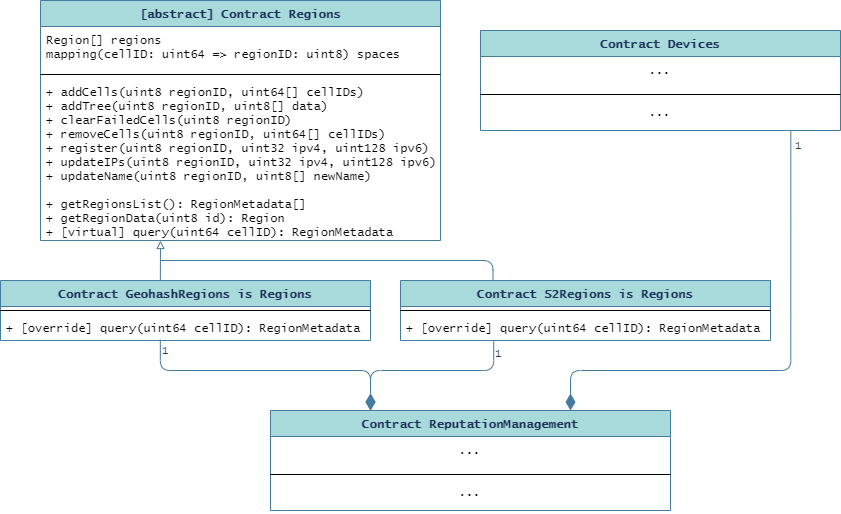
\includegraphics[width=\textwidth]{images/ContractsDeveloped.png}
  \caption{Updated \hyperref[Acronym-UML]{UML} class diagram of the Smart Contracts for supporting both geocoding techniques}
  \label{fig:ContractsDeveloped}
\end{figure}

\npara The Smart Contracts were successfully developed\footnote{GitHub repository: \url{https://github.com/ponlawat-w/uji_mt-contracts}}.
There are two different geocoding techniques, which are \textit{Geohash} and \textit{S2}.
Despite the different encoding algorithms between these two techniques, both of them result in a binary integer whose length indicates the hierarchical level of the cell.
In other words, the binary representation of the both techniques has the same structure.
Therefore, they can share the most of Smart Contract methods.

\npara Figure \ref{fig:ContractsDeveloped} shows the diagram of developed contracts.
The both geocoding techniques inherit the same abstract contract called \textit{Regions}, and they override the \textit{query} method which is the only function that they have a different behaviour, because geohash uses 5 bits to represent one level while S2 uses 2 bits.
The \code{Regions} contract was developed to be \textit{abstract}, which means that its instance cannot be initiated.
After that, the \code{Devices} contract and the \code{ReputationManagement} contract were developed.

\npara Because of that this thesis only proposes an architecture and the related technologies, so the generating of reputation value is not focused nor defined.
Therefore a direct feedback from the fog device is used in \code{ReputationManagement} contract just for proving that the contract can store and query for the value.
The practical implementation of the architecture will need to use these information of data quality and the feedback to calculate the real reputation index.

\subsection{Fog API}

\npara The \hyperref[Acronym-API]{API} for communicating with the Smart Contracts was developed\footnote{GitHub repository: \url{https://github.com/ponlawat-w/uji_mt-fog_api}}.
Each fog node serves an \hyperref[Acronym-API]{API} using the \hyperref[Acronym-HTTP]{HTTP} protocol, while it also communicates with the Geth instance through internal channel at a different port.
Therefore, the \hyperref[Acronym-API]{API} does not have to store the private key of the current node, but it can access the Blockchain through Web3 \hyperref[Acronym-API]{API} using a passphrase given by the key owner.
Through this, when a verified user wants to send a valid transaction through the fog node, the user must attach the correct passphrase in its \hyperref[Acronym-HTTP]{HTTP} request header, the \hyperref[Acronym-API]{API} will use this passphrase to decrypt the private key and unlock the account.

\npara When a user uses the \hyperref[Acronym-API]{API} to call a Smart Contract method, the \hyperref[Acronym-API]{API} needs to submit the contract call transaction to the Blockchain network, which is done by \textit{web3.js} library.
However, in some cases, it might take a longer time for the Blockchain node to mine a block and propagate the transaction.
In consequence, waiting too long for the transaction result might be interrupted by a request timeout response from the \hyperref[Acronym-HTTP]{HTTP} connection.
The user then receives an error even the transaction might be correctly pushed to the Blockchain in next few minutes.
To tackle this problem, in the developed \hyperref[Acronym-API]{API}, when a user calls a controller that submits a new transaction to the Blockchain, after \textit{web3.js} processes the request and submitted the transaction for mining, it instantly returns the transaction hash of the contract call instead of waiting until the transaction to be mined.
A user then can use the hash with another controller in the same \hyperref[Acronym-API]{API} to check the transaction status, whether it is in a queue, already mined, or rejected.

\subsection{Edge Device}

\npara The service provider and consumer code in the edge device was developed\footnote{GitHub repository: \url{https://github.com/ponlawat-w/uji_mt-edge_devices}}.
The \textit{ParticleRdWebServer} library allows a service provider to serve simple requests from its client.
Nevertheless, the usage of \textit{micro-ecc} library to sign a transaction sometimes work unexpectedly.
Even it can sign a transaction using the private key and can verify the signature by itself, but when the signature is submitted to the fog node, it is recognised to be an invalid signature.
The transaction submission request then gets rejected by the fog node and returned as a fail result.
This issue is solved by defining the number of tries to the edge device.
If the fog \hyperref[Acronym-API]{API} cannot verify the signature and responds with an error, the edge will sign and resubmit again and again until it accepts a successful response from the fog \hyperref[Acronym-API]{API}, or until it is out the number of tries.
From the observation, a transaction is usually successful between first and third try, with sometimes up to the fifth try, so the suggested number of attempts should be 5.
However, the developed code configured the number to be 10 for preparing for an unexpected case.

\subsection*{Experiment Reproducibility}

\npara The programming code, the randomly-generated input data, and the preliminary result in the experiments of this work were put into different GitHub repositories described in the footnotes.
According to \cite{Reproducibility}'s work regarding the reproducibility assessment of a research in \hyperref[Acronym-GIScience]{GIScience}, each assessment criterion can be assigned by a number between 0 and 3 which respectively means \textit{unavailable}, \textit{documented}, \textit{available}, and \textit{available and open}.
The self assignment of this work reproducibility level is by following:
\begin{itemize}
  \item \textbf{Input data:} 2
  \item \textbf{Methods preprocessing:} 2
  \item \textbf{Methods processing:} 3
  \item \textbf{Methods computational environment:} 1
  \item \textbf{Results:} 1
\end{itemize}

\newpage

\section{Experiment: Geocoding Techniques Comparison} \label{Results-TechniqueComparison}

\npara This section shows and interprets the result of two different geocoding techniques of \textit{Geohash} and \textit{S2}\footnote{GitHub repository of code in this experiment is available at\newline
\textit{Geohash: }\url{https://github.com/ponlawat-w/uji_mt-geohash_evaluation_test}\newline
\textit{S2: }\url{https://github.com/ponlawat-w/uji_mt-s2encoding}}.
However, there are some considerations regarding the bias possibility in the results as there are differences in the selected input levels of both techniques, as well as a different programming language used due to technical reasons.
This concern is elaborated in the following section (\textit{\ref{Results-TechniqueComparison-Concern}}), followed by the experiment result (\textit{\ref{Results-TechniqueComparison-Results}}).

\subsection{General Concern and Bias Consideration} \label{Results-TechniqueComparison-Concern}

\begin{table}[htb!]
  \centering
  \begin{tabular}{|c|c|r||c|c|r|}
    \hline
    \textbf{Geohash} & Bit & Cell Size & \textbf{S2} & Bit & Cell Size \\
    \hline
    1 & 5 & 12,588,175.24 km\textsuperscript{2} & 0 & 4 & 85,011,012.19 km\textsuperscript{2} \\
    & & & 1 & 6 & 21,252,753.05 km\textsuperscript{2} \\
    & & & 2 & 8 & 6,026,521.16 km\textsuperscript{2} \\
    2 & 10 & 786,760.95 km\textsuperscript{2} & 3 & 10 & 1,646,455.50 km\textsuperscript{2} \\
    & & & 4 & 12 & 413,918.15 km\textsuperscript{2} \\
    3 & 15 & 12,293.14 km\textsuperscript{2} & 5 & 14 & 104,297.91 km\textsuperscript{2} \\
    & & & 6 & 16 & 26,113.30 km\textsuperscript{2} \\
    & & & 7 & 18 & 6,529.09 km\textsuperscript{2} \\
    4 & 20 & 768.32 km\textsuperscript{2} & 8 & 20 & 1,632.45 km\textsuperscript{2} \\
    & & & 9 & 22 & 408.12 km\textsuperscript{2} \\
    5 & 25 & 12.01 km\textsuperscript{2} & 10 & 24 & 102.03 km\textsuperscript{2} \\
    & & & 11 & 26 & 25.51 km\textsuperscript{2} \\
    & & & 12 & 28 & 6.38 km\textsuperscript{2} \\
    6 & 30 & 0.75 km\textsuperscript{2} & 13 & 30 & 1.59 km\textsuperscript{2} \\
    & & & 14 & 32 & 0.40 km\textsuperscript{2} \\
    7 & 35 & 11,723.65 m\textsuperscript{2} & 15 & 34 & 99,638.93 m\textsuperscript{2} \\
    & & & 16 & 36 & 24,909.73 m\textsuperscript{2} \\
    & & & 17 & 38 & 6,227.43 m\textsuperscript{2} \\
    8 & 40 & 732.73 m\textsuperscript{2} & 18 & 40 & 1,556.86 m\textsuperscript{2} \\
    & & & 19 & 42 & 389.21 m\textsuperscript{2} \\
    & & & 20 & 44 & 97.30 m\textsuperscript{2} \\
    9 & 45 & 11.45 m\textsuperscript{2} & 21 & 46 & 24.33 m\textsuperscript{2} \\
    & & & 22 & 48 & 6.08 m\textsuperscript{2} \\
    10 & 50 & 0.72 m\textsuperscript{2} & 23 & 50 & 1.52 m\textsuperscript{2} \\
    & & & 24 & 52 & 0.38 m\textsuperscript{2} \\
    11 & 55 & 111.81 cm\textsuperscript{2} & 25 & 54 & 950.23 cm\textsuperscript{2} \\
    & & & 26 & 56 & 237.56 cm\textsuperscript{2} \\
    & & & 27 & 58 & 59.39 cm\textsuperscript{2} \\
    12 & 60 & 6.99 cm\textsuperscript{2} & 28 & 60 & 14.85 cm\textsuperscript{2} \\
    & & & 29 & 62 & 3.71 cm\textsuperscript{2} \\
    13 & 65 & 0.11 cm\textsuperscript{2} & 30 & 64 & 0.93 cm\textsuperscript{2} \\
    \hline
  \end{tabular}
  \caption{Maximum error (cell size) of different levels in Geohash and S2 Geocoding Techniques}
  \label{tab:GeohashS2Size}
\end{table}

\npara There are two issues needed to be concerned in this comparison experiment.
Firstly, the popular Geohash is based on base32 representation, despite the fact that its binary notation allows level increasing by 2 bits as S2 does, but the common Geohash libraries support only base32 manipulation.
Hence, increasing one level in a Geohash cell adds 5 more bits, but it adds 2 bits in case of S2.
The consequence is that there are no such levels where these two techniques provide a similar accuracy, and yet they cannot be fairly compared.

\npara Table \ref{tab:GeohashS2Size} shows the comparison of a cell area size between Geohash and S2 in different levels\footnote{
  \npara Geohash accuracy:\newline\href{https://stackoverflow.com/questions/13448595/geohash-string-length-and-accuracy}{\code{https://stackoverflow.com/questions/13448595/\newline
geohash-string-length-and-accuracy}}\newline
  \npara S2 cell statistics: \url{https://s2geometry.io/resources/s2cell_statistics}
}.
From the table it can be observed that at the same bit length, Geohash has a smaller cell size which means it provides more precision than S2 at the same length.
We can note that the number of S2 bits shown in the table includes the end bit of \code{1} which is insignificant for interpreting the coordinates.
For this reason, before going to compare these two techniques it needs to decide the factor for paring the levels, for example to be based on data length or cell size.
Since the Smart Contracts in this work store geocoded cells in a fixed-length integer of 64 bits, the number of bits stored is not concerned regardless of its level; therefore it compared between those levels whose area size are most similar, which are:

\begin{itemize}
  \item Geohash level 4 and S2 level 9
  \item Geohash level 5 and S2 level 12
  \item Geohash level 6 and S2 level 14
  \item Geohash level 7 and S2 level 16
\end{itemize}

Secondly, another consideration is the possible bias regarding the calculation time.
As the proposed architecture is based on JavaScript for the aforementioned reason, the library used for encoding the areas will also be developed in JavaScript.
However, there is no any S2 region covering libraries available in JavaScript library database as of found.
The official S2 library is available in C++, Go language and Python.
Go language is selected for this comparison.
This leads to the consideration that Go language is a compiled language, while JavaScript is an interpreted language; this programming language selection might affect the comparison quality.

\subsection{Comparison Results} \label{Results-TechniqueComparison-Results}

\subsubsection*{File size}

\begin{figure}[htb!]
  \centering
  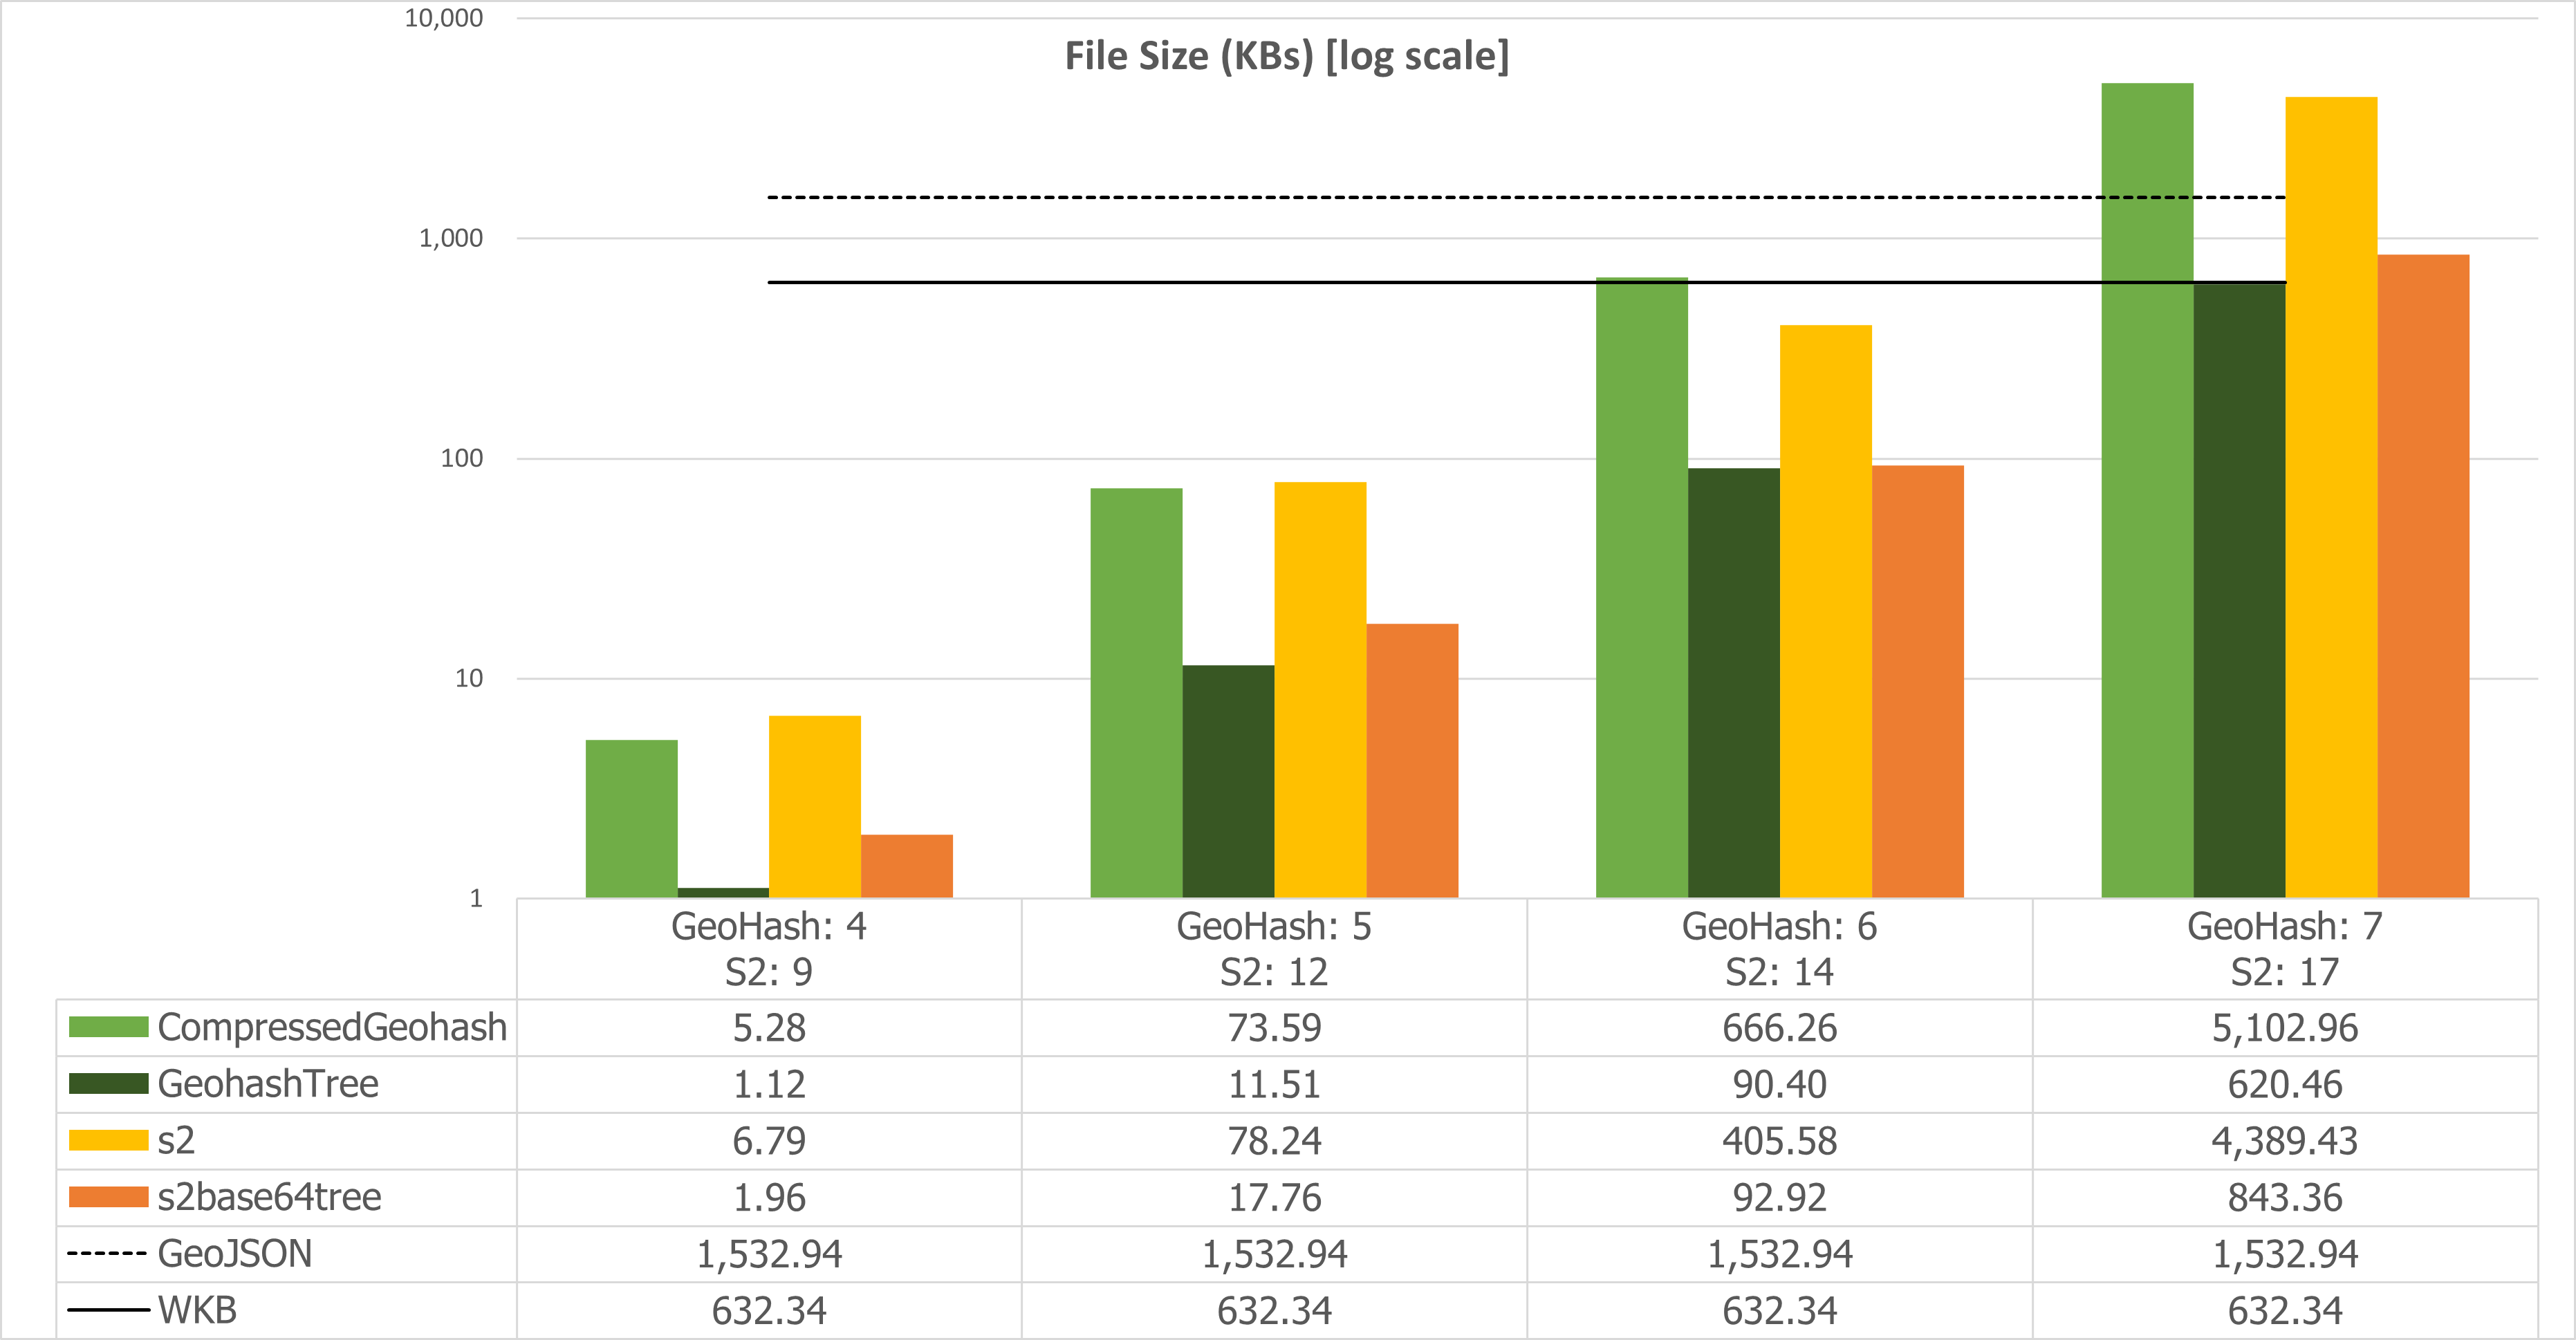
\includegraphics[width=\textwidth]{images/ResultsGSFileSize.png}
  \caption{Graph showing the file size (in kilobytes) comparison between Geohash and S2 technqiues}
  \label{fig:ResultsGSFileSize}
\end{figure}

\npara Figure \ref{fig:ResultsGSFileSize} shows the size in kilobytes of resulted geocoded cells, using the administrative region polygons in Spain as the input data.
The stable horizontal lines, black solid and dashed, are sizes of original polygons in \textit{Well-Known Binary (\hyperref[Acronym-WKB]{WKB})} and Geo\hyperref[Acronym-JSON]{JSON} respectively.
The row \code{CompressedGeohash} and \code{S2} shows the file sizes of the cell ID lists in each technique.
The row \code{GeohashTree} and \code{s2base64tree} shows the file sizes of compressed cell ID lists using the proposed algorithm.
The Graph is shown in the logarithm scale.
The result shows a very similar file size between Geohash and S2 for preserving a similar precision.
It also shows that the proposed compressing algorithm can significantly reduce the size from the prefix-redundant list.
It also demonstrates that using compressed Geohash level 6 or S2 level 14 can save disk space than the original polygonal data, but for the next level, both techniques consume a larger space than the \hyperref[Acronym-WKB]{WKB} data.

\subsubsection*{Number of Resulted Cells}

\begin{figure}[htb!]
  \centering
  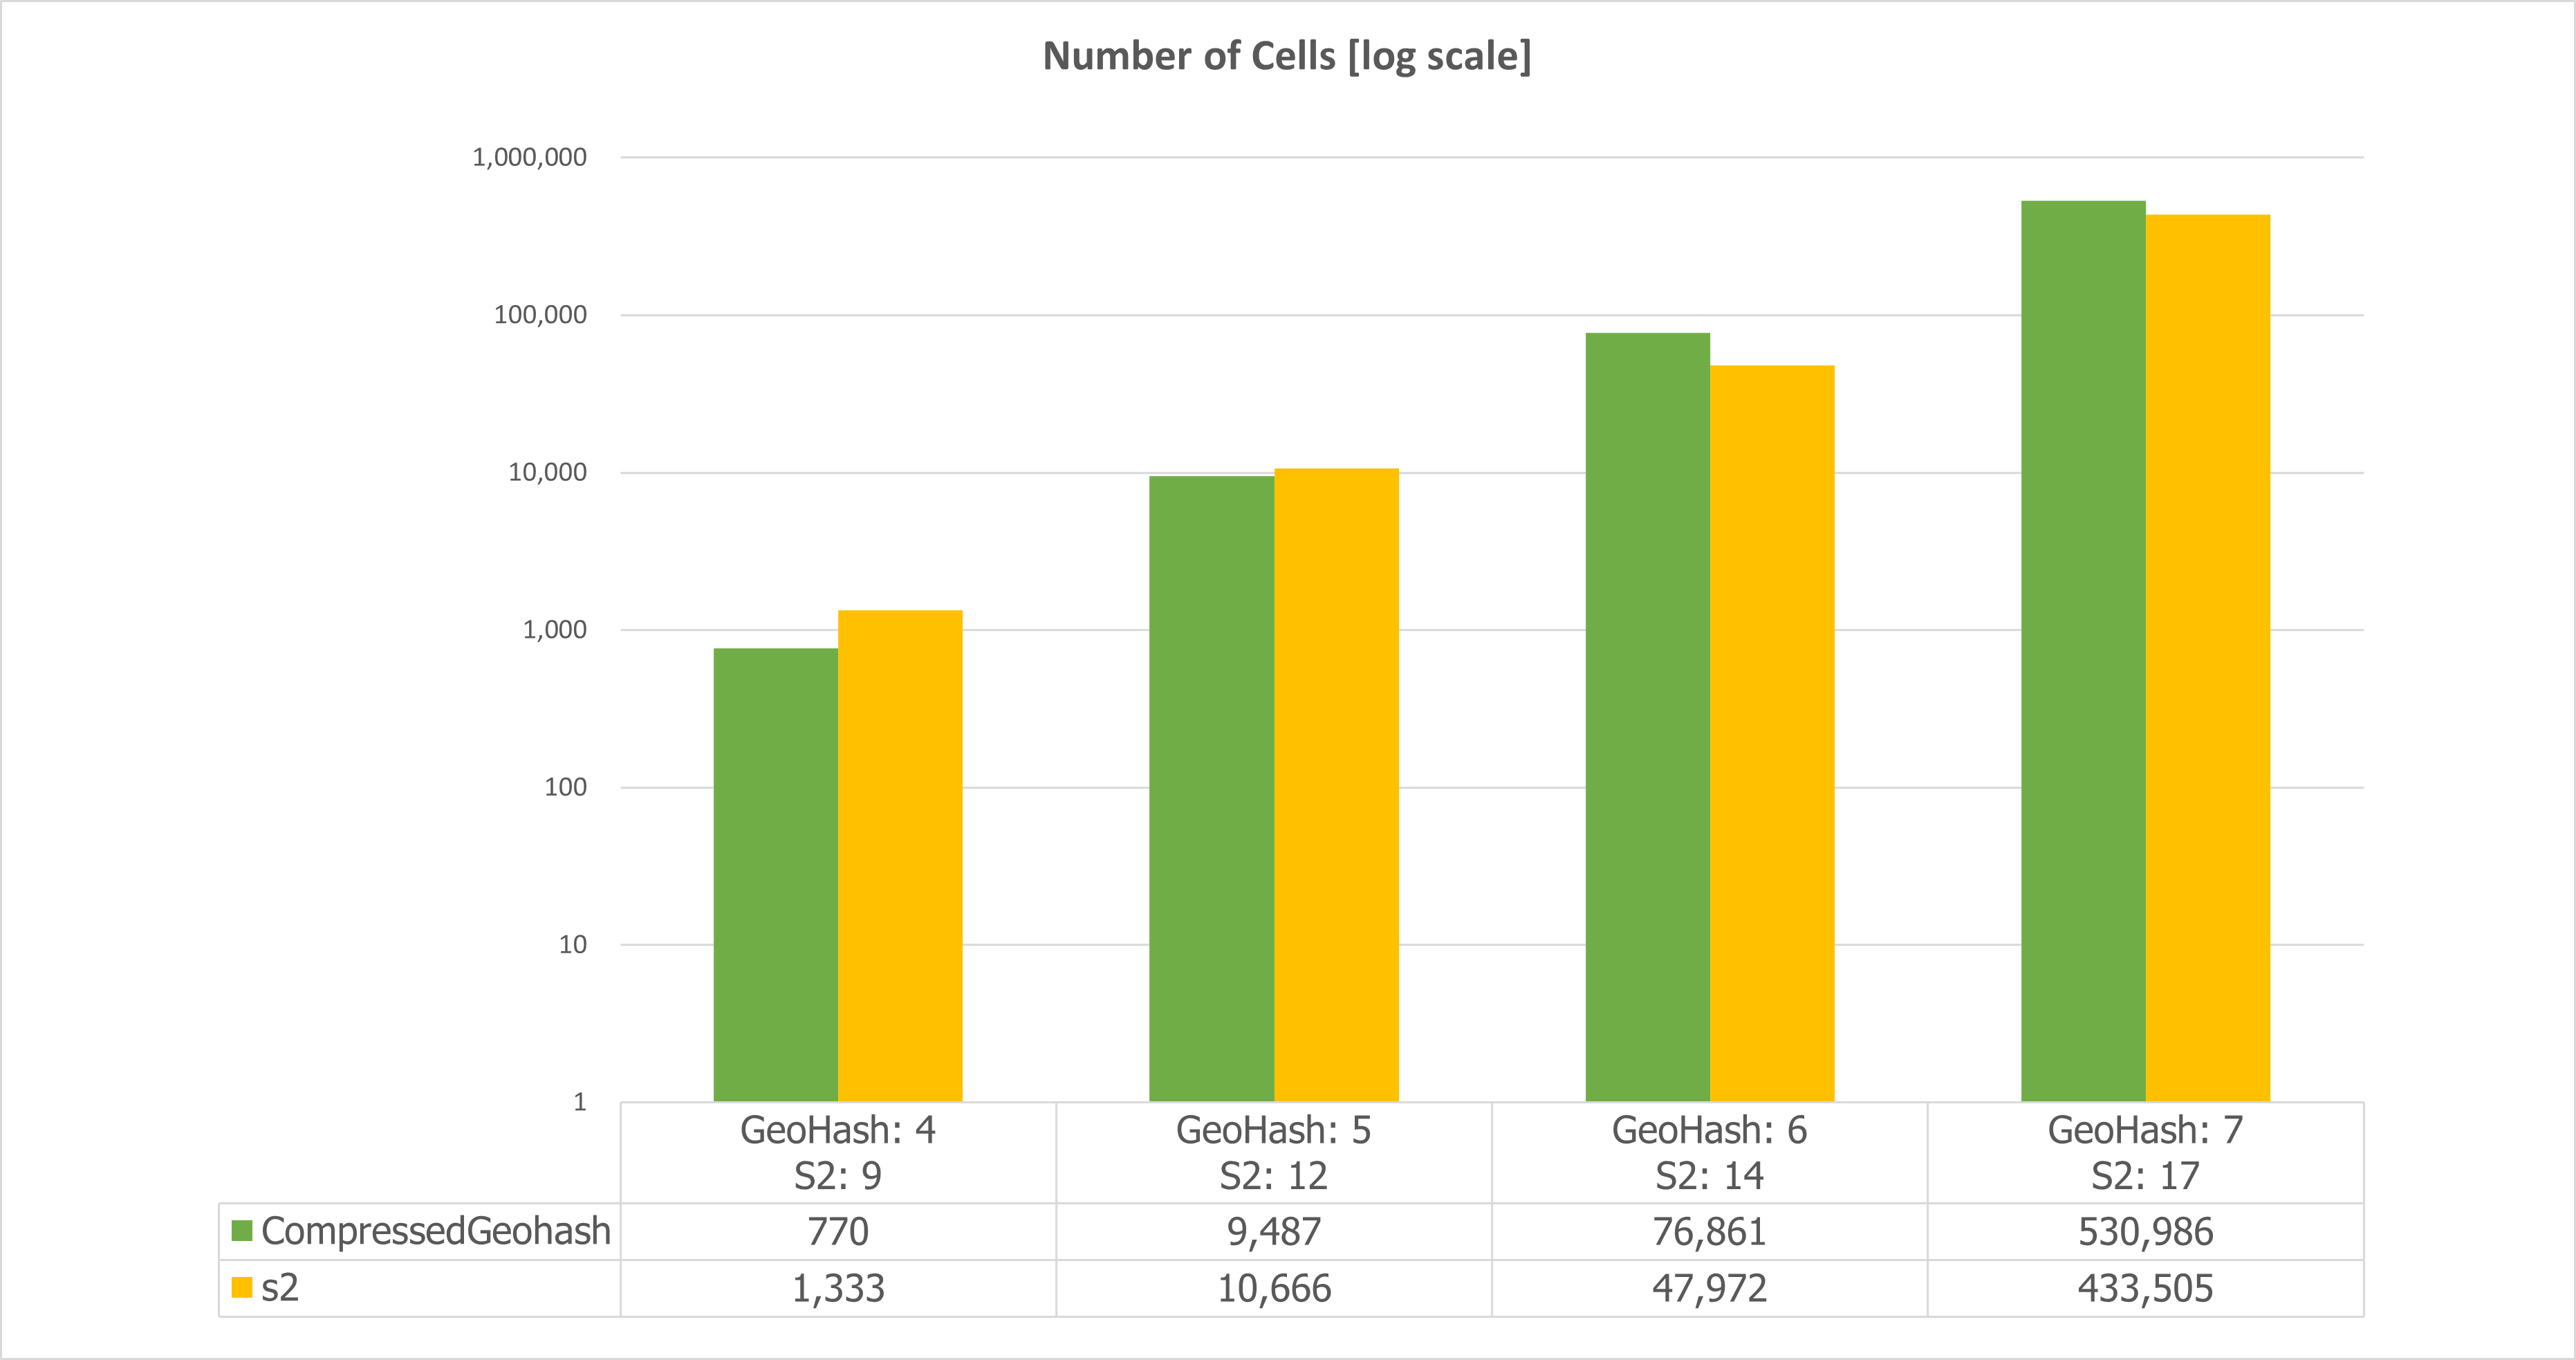
\includegraphics[width=\textwidth]{images/ResultsNumCells.png}
  \caption{Graph showing the number of cells resulted from fitting areas to geocoded cells using Geohash and S2 techniques}
  \label{fig:ResultsNumCells}
\end{figure}

\npara Figure \ref{fig:ResultsNumCells} shows the number of cells outputted from Geohash and S2 geocoding techniques.
The graph is displayed using a logarithm scale.
From the graph, it can be observed that Geohash and S2 resulted in a similar number of cells, but they are uncertain for defining which one is better, as S2 contains more number of cells in the lower level, while in the higher-level Geohash requires more.
The reason could be caused by the characteristics of the input data, such as the alignment of the input polygons.

\subsubsection*{Calculation Time}

\begin{figure}[htb!]
  \centering
  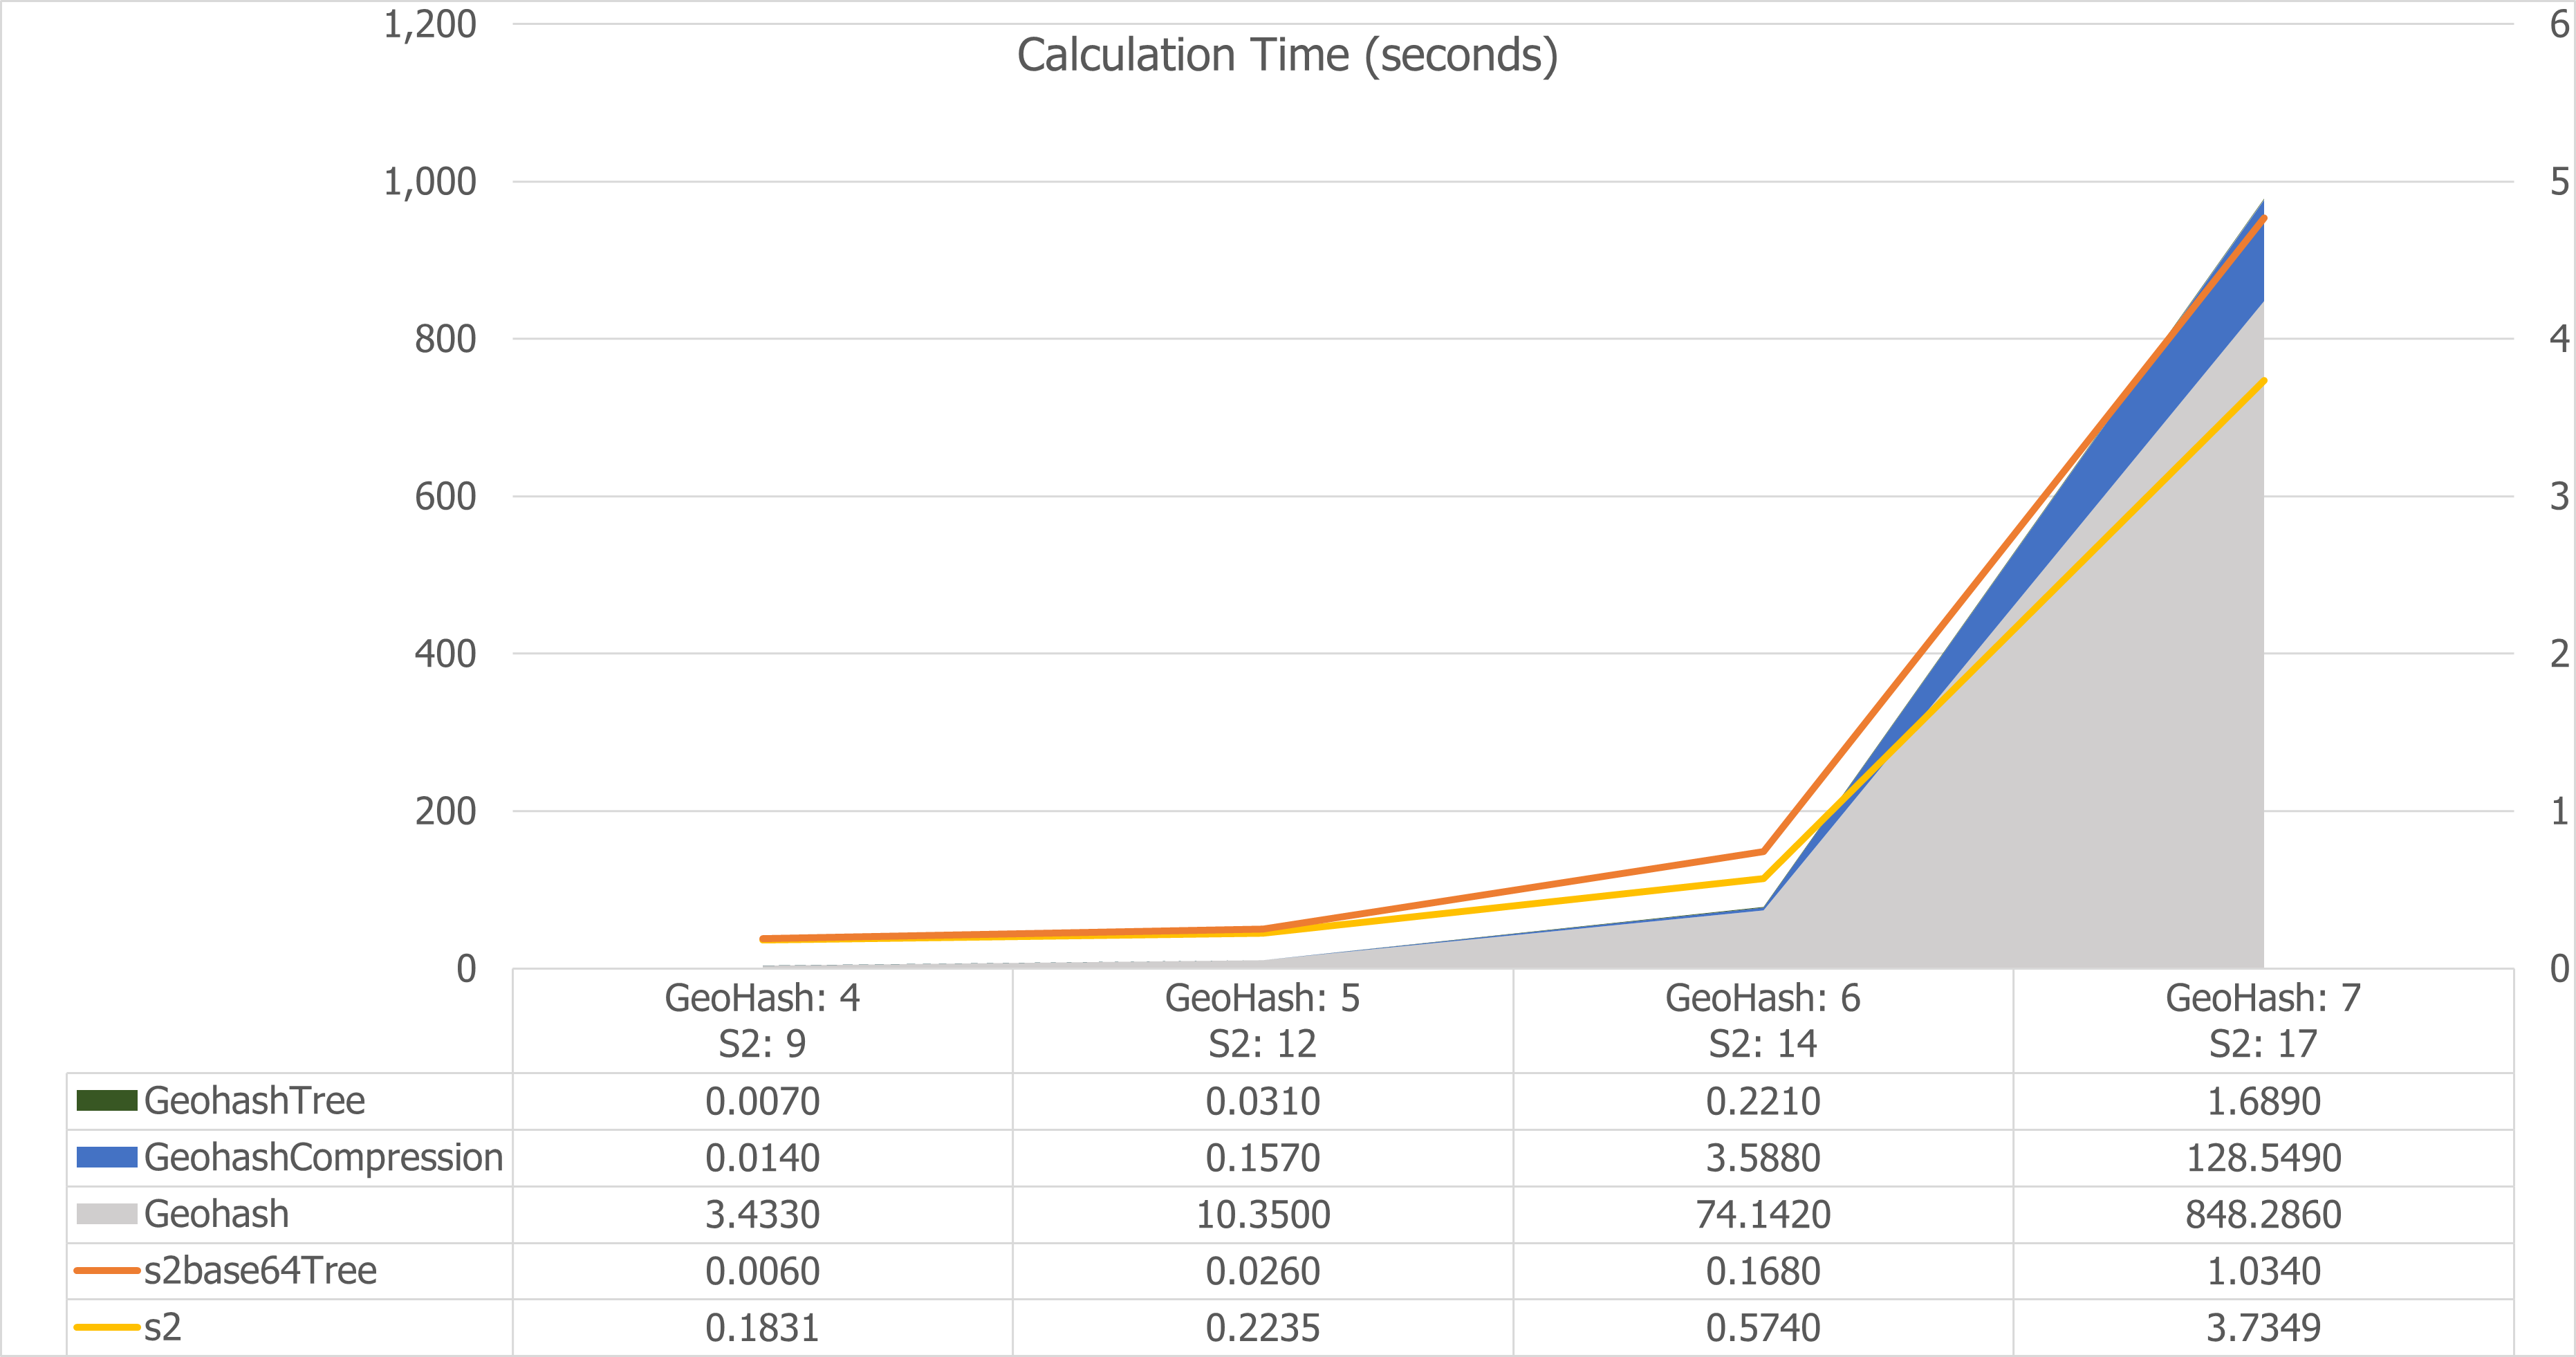
\includegraphics[width=\textwidth]{images/ResultsGSCalculationTime.png}
  \caption{Graph showing calculation time for geocoding and compressing the data using Geohash and S2 techniques}
  \label{fig:ResultsGSCalculationTime}
\end{figure}

\npara Figure \ref{fig:ResultsGSCalculationTime} shows time spent for calculation in geocoding the polygons using Geohash and S2 techniques.
The results between two techniques are too different.
The y-axis has to be split, with the left (blue) axis indicates Geohash calculation time in second, and the right (orange) indicates S2 calculation time in the same unit.
From the result, it can be observed that S2 is much faster than Geohash as converting the whole areas spent less than even 10 seconds in the highest precision, while Geohash took more than ten minutes to accomplish all the tasks.
However, the reason behind this difference could be, as described in the previous section (\textit{\ref{Results-TechniqueComparison-Concern}}), that they used a different programming language.
Furthermore, the library used for fitting the polygons into S2 cells is the official library developed by the S2 developer team, but the Geohash library is developed by a third-party developer.
\newpage

\section{Experiment: Contract Simulation} \label{Results-Simulation}

\begin{figure}[hbt!]
  \centering
  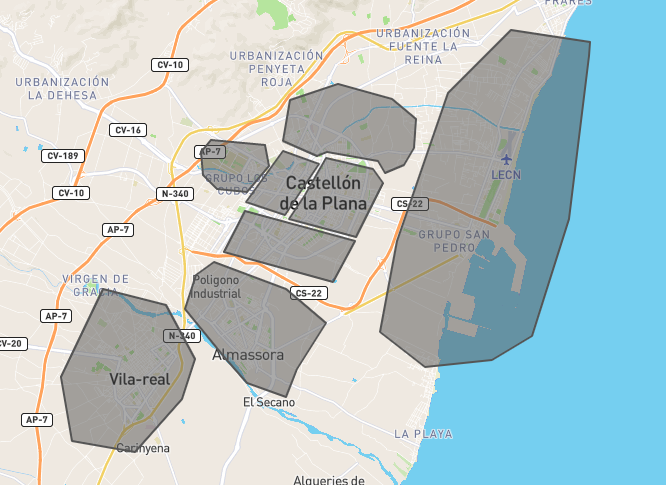
\includegraphics[width=\textwidth]{images/ExperimentInput.png}
  \caption{The region divisions of data used in the simulation experiment}
  \label{fig:ExperimentInput}
\end{figure}

\npara This section shows the simulation results of deploying the smart contracts into the Ethereum network.
There are four experiments in this section, which are 1) gas consumption in the contract deployment, 2) interacting performance with the contracts, and 3) mining performance of the devices in the system.

\npara Figure \ref{fig:ExperimentInput} shows the region divisions of data used in this experiment.
The locations used in querying and device mobility assessment in this experiment are randomly generated within these regions.

\subsection*{Gas Consumption in the Contract Deployment}

\begin{figure}[htb!]
  \centering
  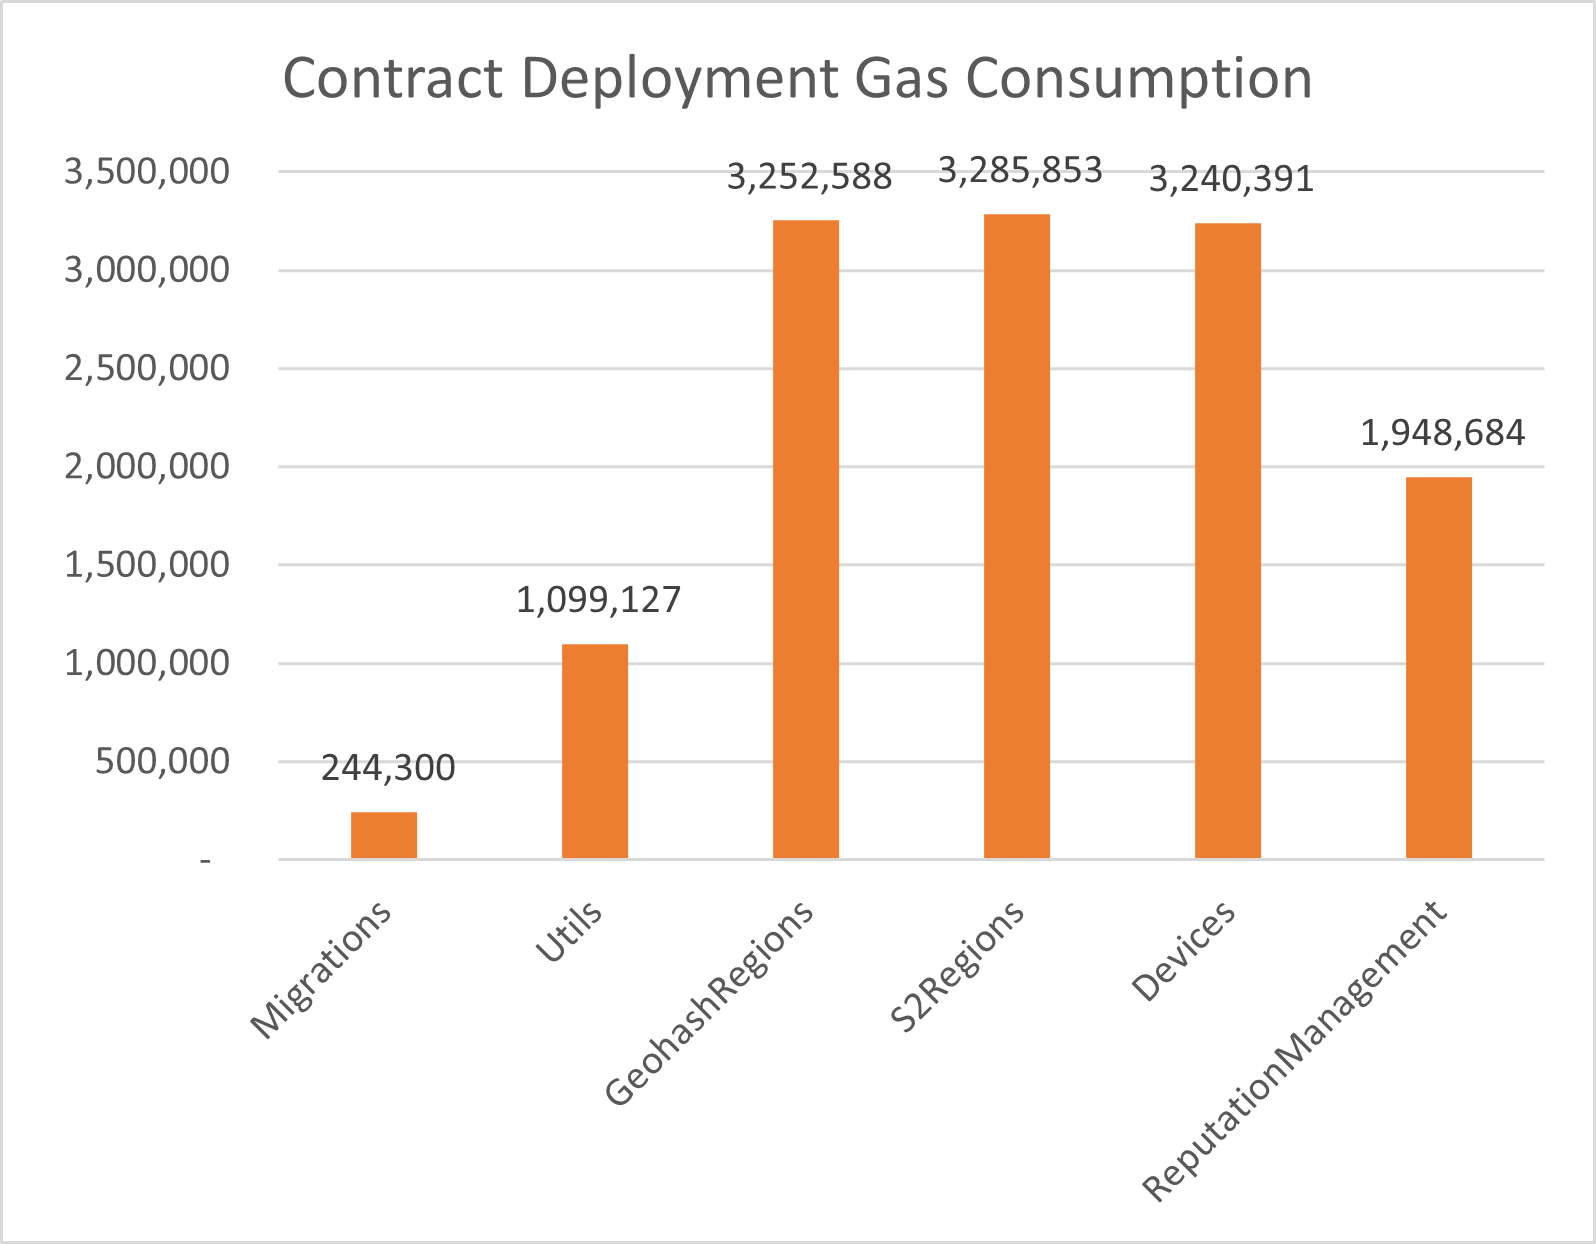
\includegraphics[width=\textwidth]{images/ExperimentDeploy.png}
  \caption{Gas consumption in contracts deployment}
  \label{fig:ExperimentDeploy}
\end{figure}

\npara This experiment measures the Ethereum gas spent on deploying the developed Smart Contracts into the Ethereum Network.
Figure \ref{fig:ExperimentDeploy} shows the result of the experiment.
From the result, it can be observed that \textit{Regions} and \textit{Devices} Contracts use more gas comparing to the other contracts.
This is caused from the number of methods and the computational operations in the contracts.
It can also be observed that the implementation of the regions based on \textit{S2} geocoding technique consumes slightly more gas than the \textit{Geohash} one.
The reason behind this difference could be that the operations in S2 have to handle the end bit of the cell when changing the level, while the action is unnecessary in Geohash.

\subsection*{Interacting Performance with the Regions Contracts}

\npara This experiment added a number of example regions data (Figure \ref{fig:ExperimentInput}) into the Smart Contracts that use Geohash and S2.
The design of this experiment divided data inputs into three different levels.
In case of Geohash, the maximum cell lengths are 6, 7, and 8.
And in case of S2, they are 14, 17, and 19.
However, the Smart Contracts returned an \textit{out of gas} error when trying to add the regions of the third level in the both techniques (Geohash: 8, S2: 19).
For this reason, this experiment results will only show the first two lengths:

\begin{itemize}
  \item \textbi{Geohash Precision 1}: 6
  \item \textbi{Geohash Precision 2}: 7
  \item \textbi{S2 Precision 1}: 14
  \item \textbi{S2 Precision 2}: 17
\end{itemize}

\begin{figure}[htb!]
  \centering
  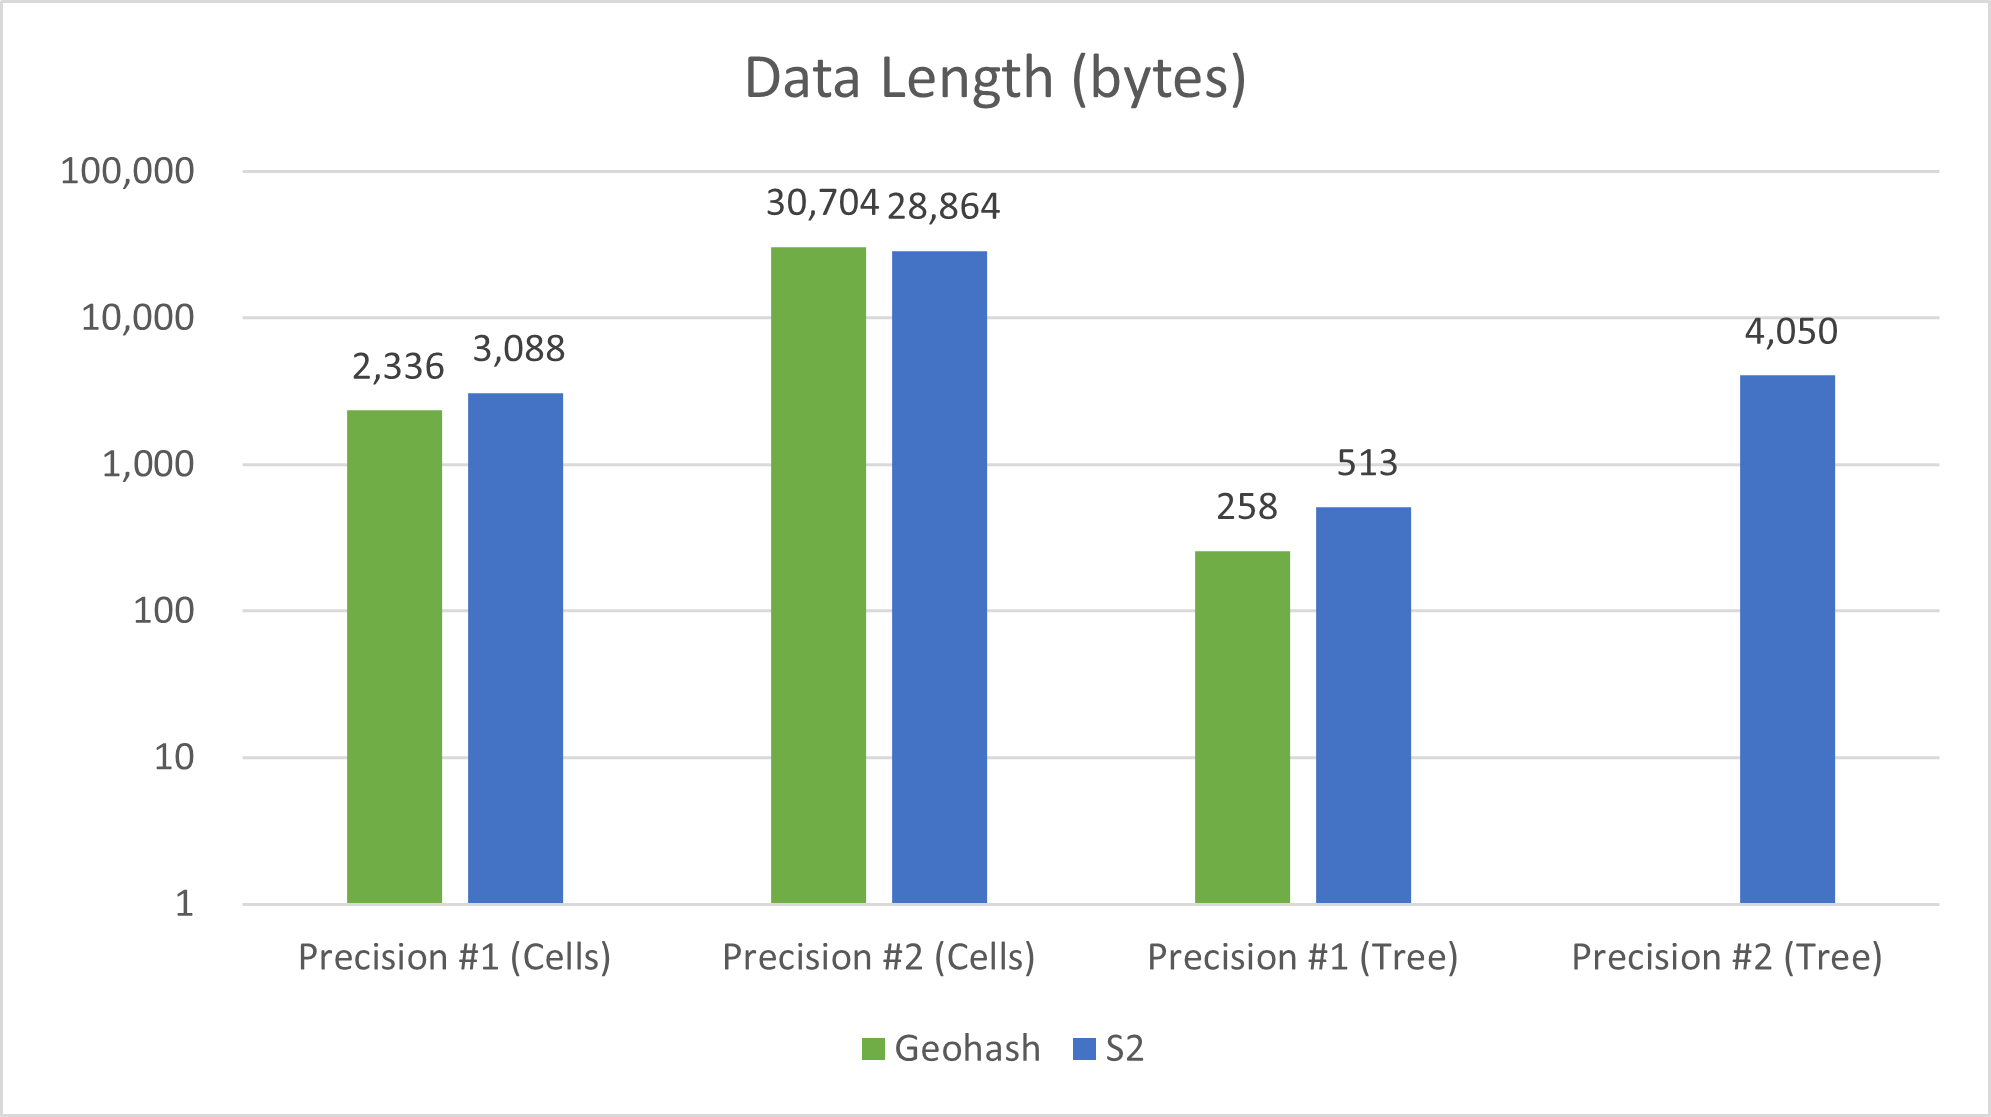
\includegraphics[width=\textwidth]{images/ExperimentRegionsLength.png}
  \caption{Graph showing the sizes of the input data used for adding new regions into the contracts}
  \label{fig:ExperimentRegionsLength}
\end{figure}

\begin{figure}[htb!]
  \centering
  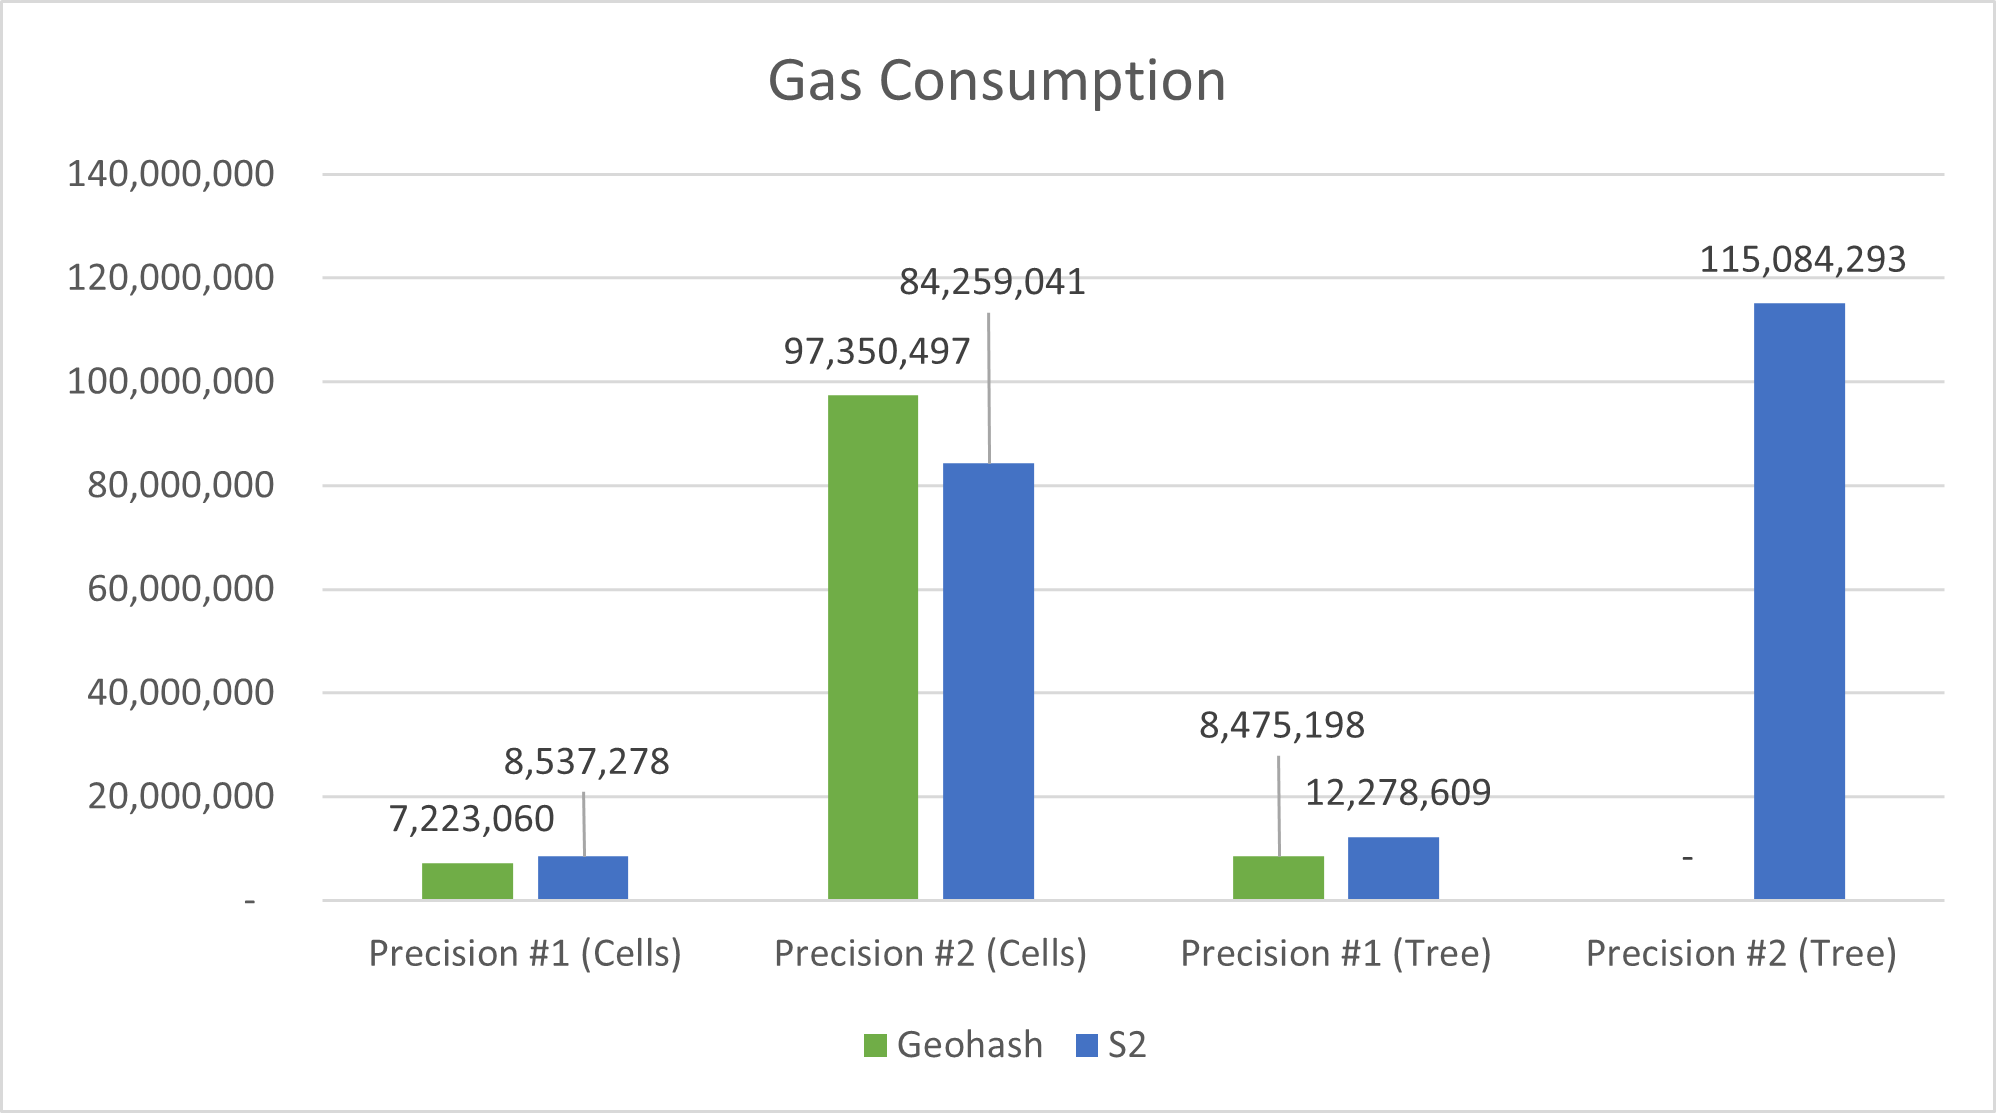
\includegraphics[width=\textwidth]{images/ExperimentRegionsGas.png}
  \caption{Graph showing gas consumption when adding new regions into the contracts}
  \label{fig:ExperimentRegionsGas}
\end{figure}

\begin{figure}[htb!]
  \centering
  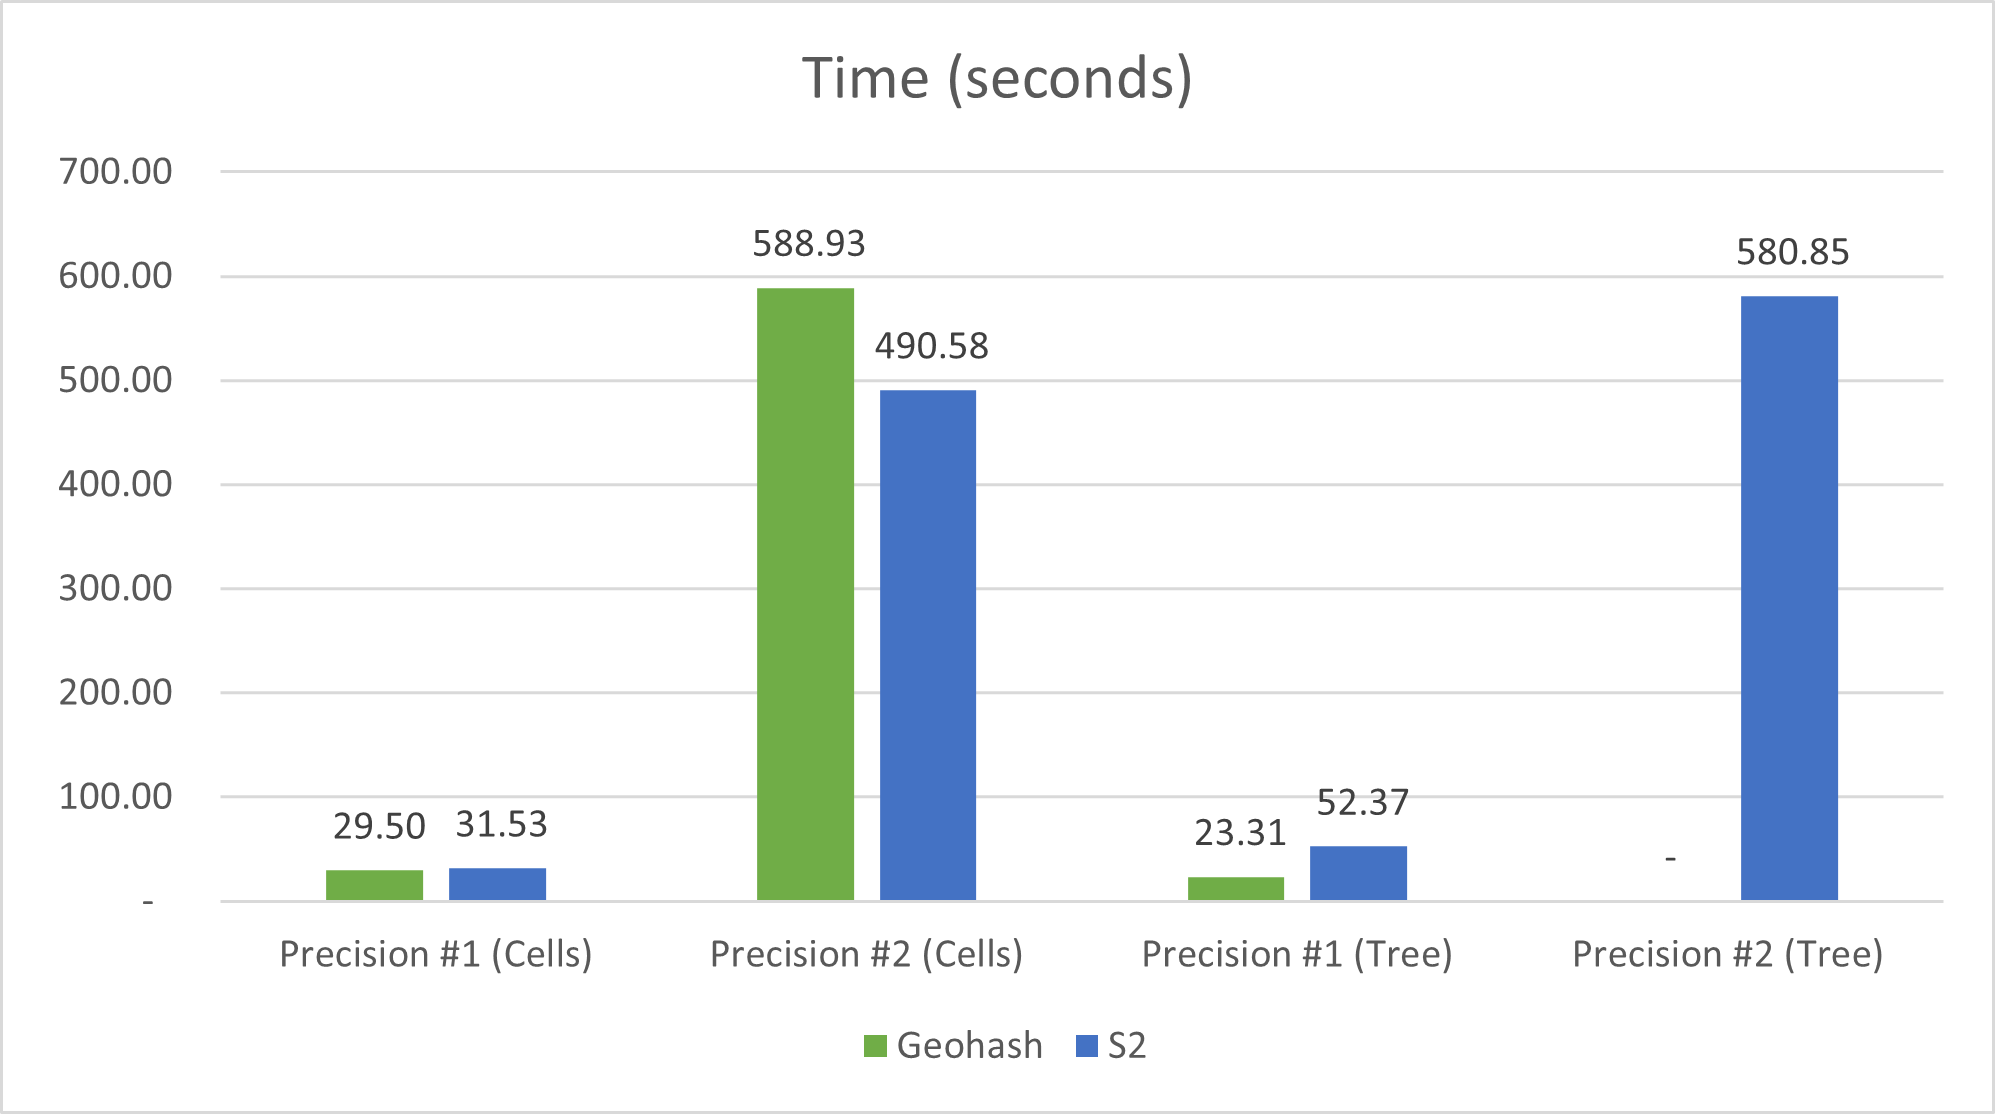
\includegraphics[width=\textwidth]{images/ExperimentRegionsTime.png}
  \caption{Graph showing time spent when adding new regions into the contracts}
  \label{fig:ExperimentRegionsTime}
\end{figure}

\npara Figure \ref{fig:ExperimentRegionsLength} shows the input data lengths of the different regions contracts implementation.
The precision \verb|#|2 of Geohash tree returned an error of \textit{out of gas}, therefore it cannot be included to the result graph.
From the result it can be observed that the sizes of tree-based compressed input data are significantly less than the cell lists.

\npara Figure \ref{fig:ExperimentRegionsGas} shows gas consumption when adding the regions into the Smart Contract.
Despite their significant smaller size of input data, adding data using the trees consumes more gas than using only an array of geocoded cells.
A possible reason is that using Ethereum to expand the tree causes an additional cost of computation.

\npara Figure \ref{fig:ExperimentRegionsTime} shows time spent to add the regions data into the Smart Contract.
It can be observed that in some cases tree-base input data spends more time than cells array but it results in another way in the other cases.
There might be another factor that affects the calculation time in this experiment, however, by the current result data it is difficult to conclude which one is faster.

\begin{figure}[htb!]
  \centering
  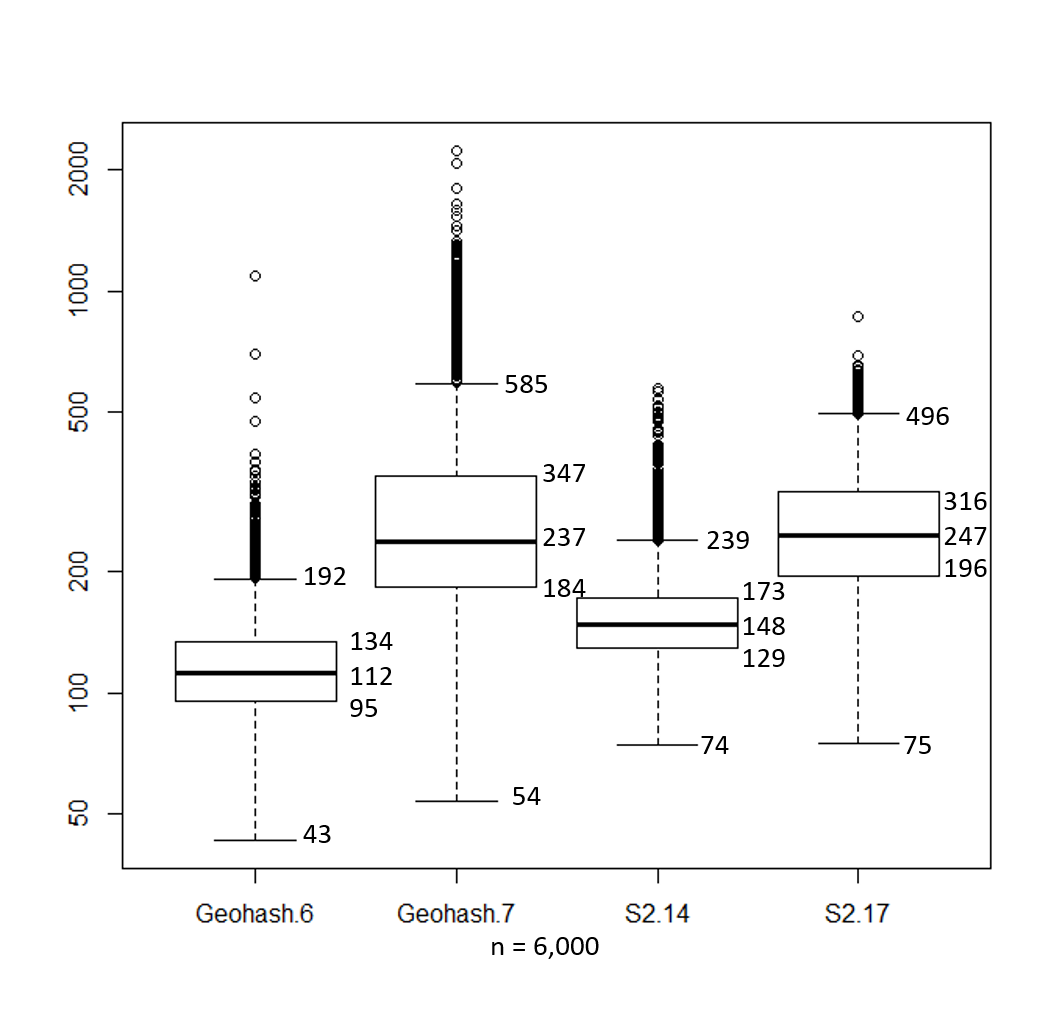
\includegraphics[width=\textwidth]{images/ExperimentQuery.png}
  \caption{Graph showing time spent when querying for a cell in the contracts (in millisecond)}
  \label{fig:ExperimentQuery}
\end{figure}

\npara The last experiment is the query experiment.
This experiment randomly generated 6,000 points in the space and used the same data set to test the query time in the Smart Contracts based on Geohash and S2.
In these 6,000 points, 5,000 of them are belong to an existing region in the Smart Contracts, the other 1,000 are the points that do not fall into any region.
Figure \ref{fig:ExperimentQuery} shows a boxplot of the experiment results.
From the results, it can be observed that in the similar level, querying for a cell in Geohash is slightly faster than S2.
The reason can be that one level of a Geohash cell requires 5 bits of data while S2 requires 2 bits.
For this reason, to query for a cell over the data, Geohash requires 7 iterations to check across all the levels and S2 requires up to 32 iterations to check.

\subsection*{Mining Performance of the Devices in the System}

\begin{figure}[htb!]
  \centering
  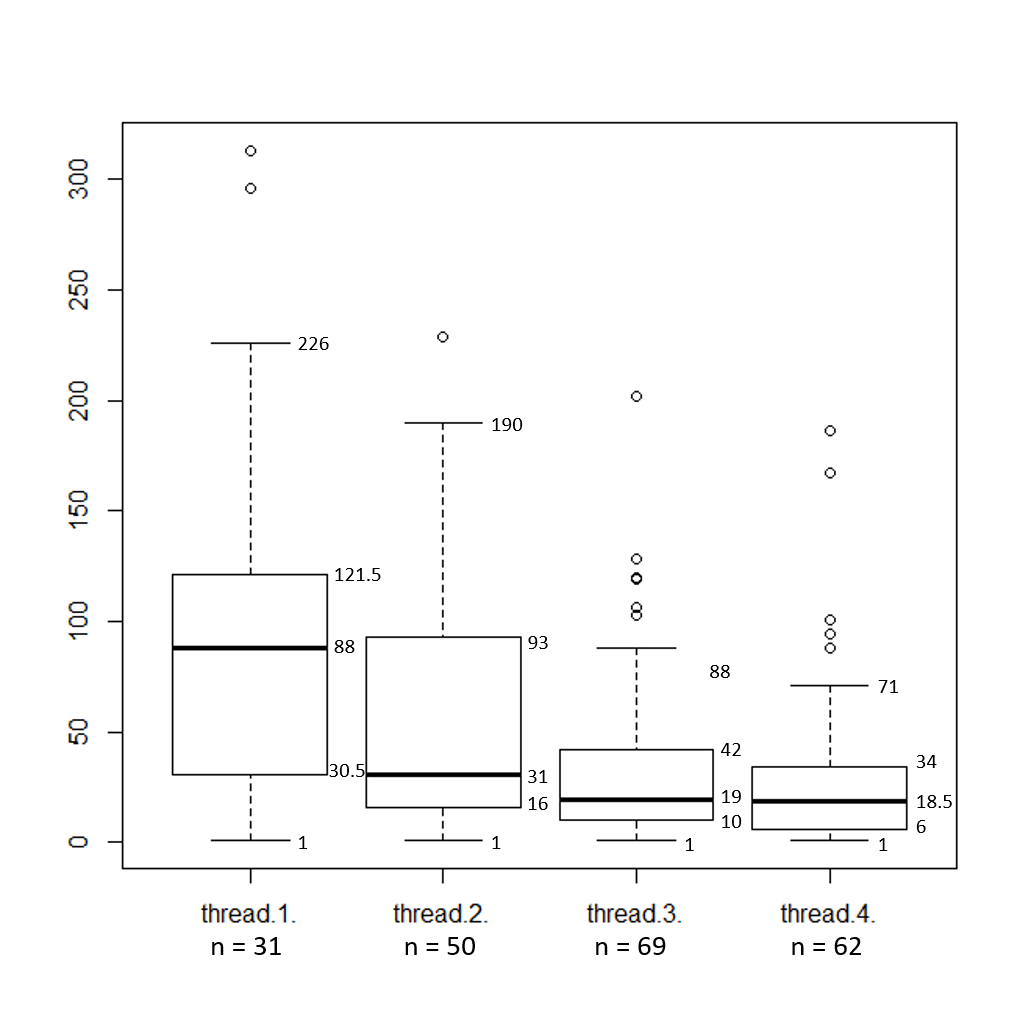
\includegraphics[width=\textwidth]{images/ExperimentMining.png}
  \caption{Graph showing time spent when mining a new block into the chain (in second)}
  \label{fig:ExperimentMining}
\end{figure}

\npara This experiment was designed to compare the possibility and performance of the Ethereum nodes using IoT devices when mining a new block to the chain.
It compares a personal computer of 4-core \hyperref[Acronym-CPU]{CPU} and a Raspberry Pi which is used as a fog device.
However, due to hardware limitation, the Raspberry Pi did not manage to mine any block.
Instead, it returned an out of memory error and halted the Ethereum client.
For this reason, despite the fact that Raspberry Pi can be a node in Ethereum network and can submit the transactions, it cannot be a miner to publish the chain.
A possible solution to this issue is to modify the implementation of the Ethereum network to use a different consensus algorithm, whose default is Proof-of-Work, to be the Proof-of-Authority algorithm\footnote{\hyperlink{https://ethereum.stackexchange.com/questions/24955/geth-mining-on-32bits-host-raspberry-pi-memory-error}{\code{https://ethereum.stackexchange.com/questions/24955/\newline
geth-mining-on-32bits-host-raspberry-pi-memory-error}}}.
However, this experiment continued to measure the mining time using only the personal computer running on the different thread numbers, keeping the default consensus algorithm which is Proof-of-Work.
Figure \ref{fig:ExperimentMining} shows the results of the experiment.
As expected, using more thread tends to spend less time to mine a block into the chain.
The mining time indicates time needed to publish a transaction into the network.
Hence, from the results it can take up to minutes for a change in the Smart Contract to be propagated over the network.
\newpage

\section{Experiment: Deployment and Scenario} \label{Results-Deployment}

\npara This sections describes the results and related discussions after having deployed the proposed architecture into the real \hyperref[Acronym-IoT]{IoT} devices.

\subsection*{Fog Layer}

\begin{figure}[hbt!]
  \centering
  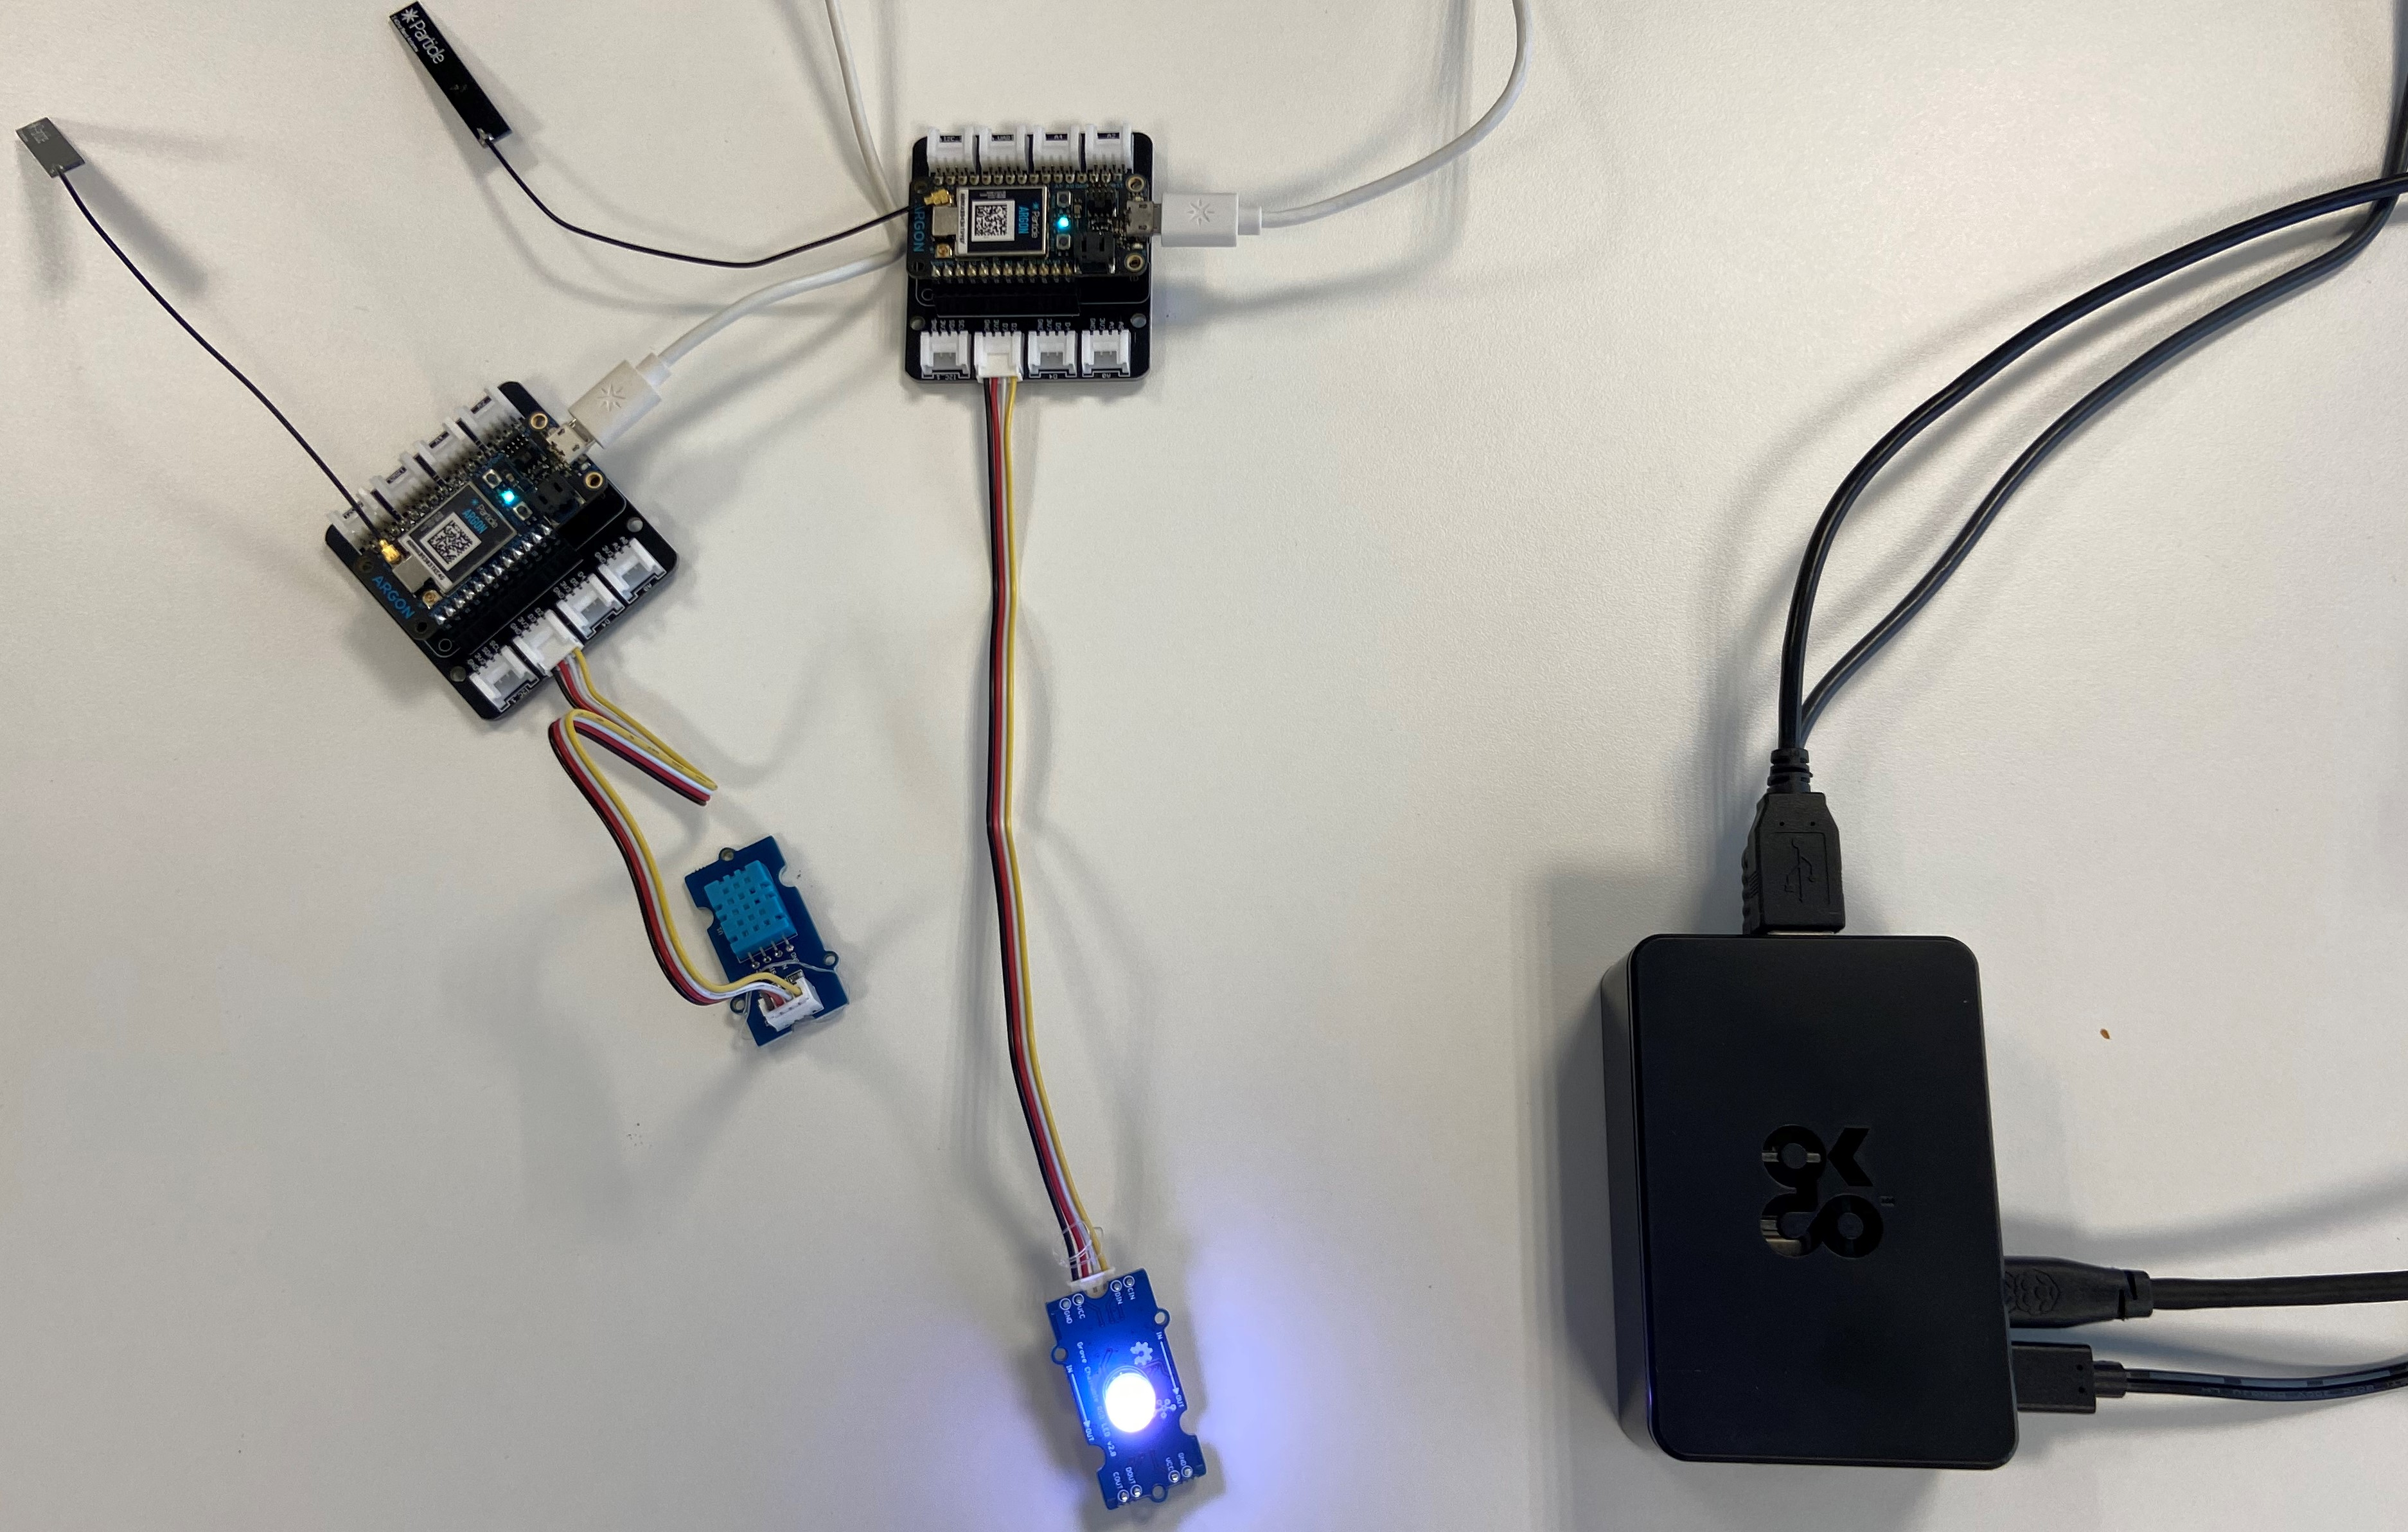
\includegraphics[width=\textwidth]{images/ScenarioBlue.jpg}
  \caption{The instalment of test scenario: edge service provider, edge service consumer, fog Raspberry Pi}
  \label{fig:ScenarioBlue}
\end{figure}

\npara The \hyperref[Acronym-API]{API}s and a Geth client were installed into a Raspberry Pi 4.
After using the API to interact with the Smart Contracts, it showed that the Raspberry Pi 4 has enough potential to serve as an \hyperref[Acronym-API]{API} and run an Ethereum node at the same time.
The Raspberry Pi, whose operating system is based on Linux, is also able to run another service, including \hyperref[Acronym-SSH]{SSH}, which allows a remote access to the device.
Hence, it is not necessary to be physically with the node in order to maintain, update or configure it.
The shell script\footnote{GitHub repository: \url{https://github.com/ponlawat-w/uji_mt-raspi_scripts}} enables Raspberry Pi to run the \hyperref[Acronym-API]{API} and Geth client as a service, therefore it is simpler for the administrator to access the device via \hyperref[Acronym-SSH]{SSH} and execute the service command in order to start, stop the service, as well as diagnose it when there is a problem.
The Smart Contracts allowed the devices to register themselves with their \hyperref[Acronym-IP]{IP} address information.
Once it is added into the Blockchain, another node can also see the list of the registered fog nodes and their \hyperref[Acronym-IP]{IP} addresses, so that they can use the \hyperref[Acronym-IP]{IP} address as a \hyperref[Acronym-URL]{URL} base for the \hyperref[Acronym-API]{API}.

\npara However, in this test scenario, the registered \hyperref[Acronym-IP]{IP} addresses is in the same \hyperref[Acronym-LAN]{LAN} network.
In practice, fog node can be installed in a different area which uses a different internet network.
It might be necessary to consider using another service to forward device \hyperref[Acronym-IP]{IP} address or using a \hyperref[Acronym-VPN]{VPN} to let the device be accessible from outside.

\npara Figure \ref{fig:ScenarioBlue} shows the instalment of this test experiment.
The Raspberry Pi who acts as a fog node is located as a black box in the right side of the image.

\subsection*{Edge Layer}

\begin{figure}[hbt!]
  \centering
  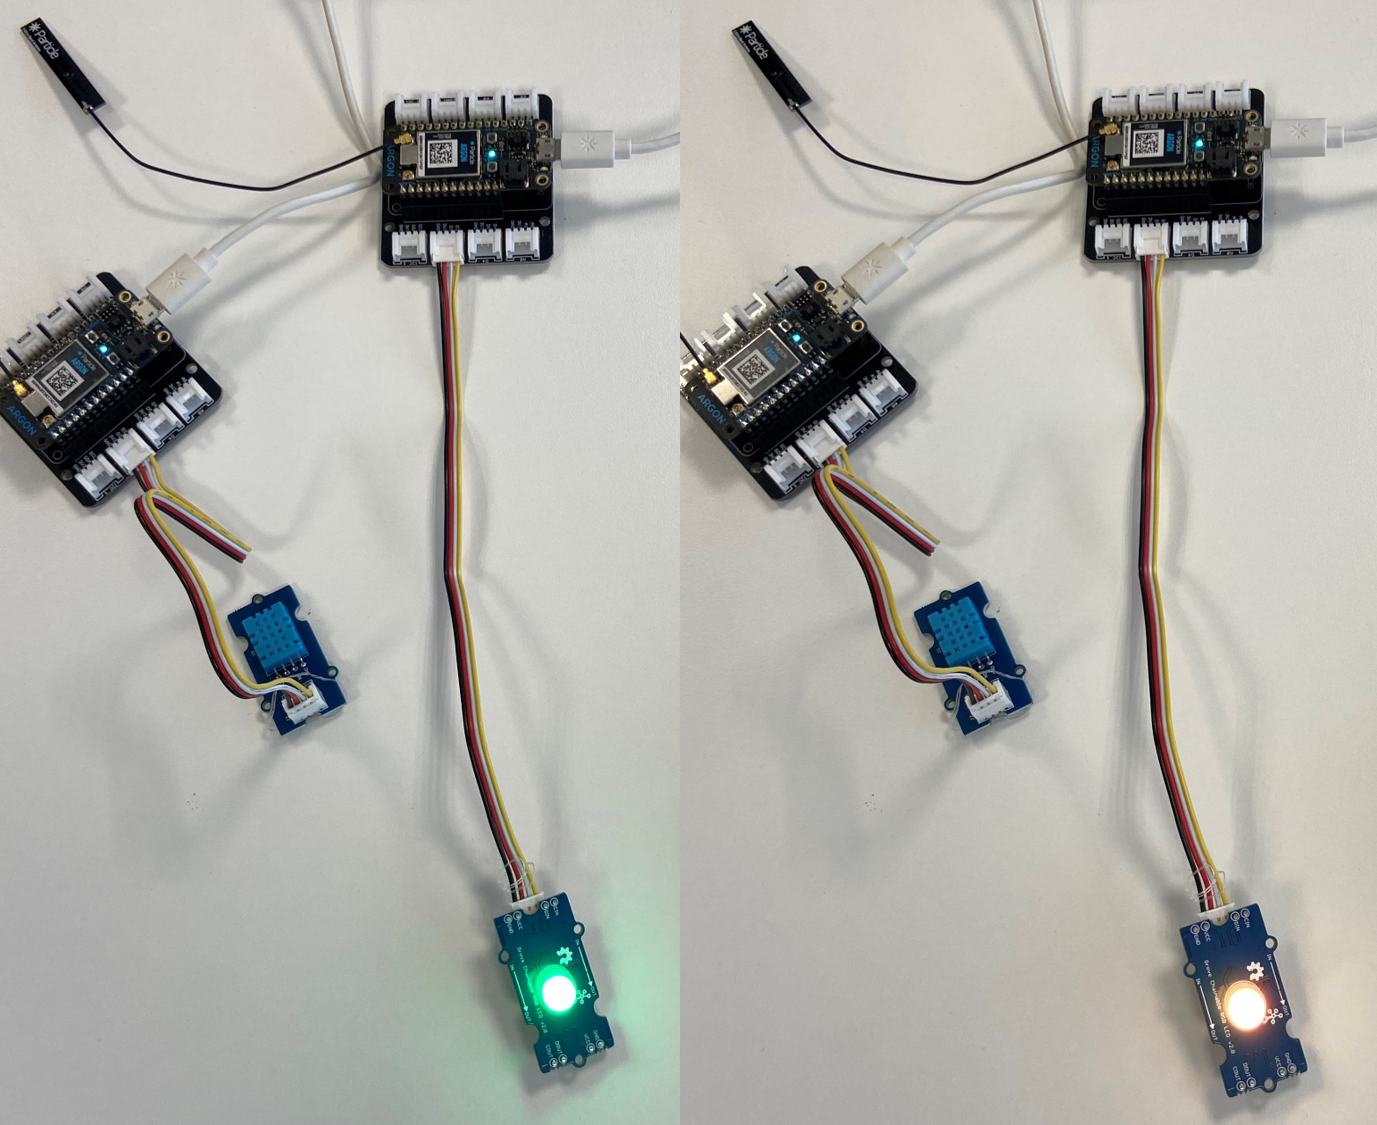
\includegraphics[width=\textwidth]{images/ScenarioGreenOrange.png}
  \caption{The service consumer status \hyperref[Acronym-LED]{LED} shows in green (trust) and orange (not trust)}
  \label{fig:ScenarioGreenOrange}
\end{figure}

\npara In the test scenario, the edge service provider was attached to a temperature and humidity sensor, and exposed the services into its device registration data.
However, due to lack of equipment, it was unfortunately not able to equip a \hyperref[Acronym-GPS]{GPS} module or any positioning module to it.
Thus, the device's position had to be simulated and manually set by the user, which is not supposed to be the case in the practical implementation.

\npara After the device had been switched on, it was able to received an Ethereum address and private key from the user, and register itself to the Smart Contracts through the fog \hyperref[Acronym-API]{API}.
To send the transaction, the device managed to sign a transaction and submit to the fog \hyperref[Acronym-API]{API}.
Using an \hyperref[Acronym-HTTP]{HTTP} caller application in the personal computer (in this case \textit{Postman}), it was able to communicate with the edge device through its \hyperref[Acronym-API]{API} served on the exposed \hyperref[Acronym-IP]{IP} address.
The \hyperref[Acronym-IP]{IP} address of the device can be discovered by query in the contract via the fog \hyperref[Acronym-API]{API}.
It was also able to query for the reputation value using fog \hyperref[Acronym-API]{API} and establish a new connection to consume the service.
The service provider returned correct values of the service, and parallelly sent the observed data to the fog node as defined in the architecture.
Finally, after finishing the service consumption, the user sent a feedback to the fog node, which was later calculated (or random in this work) to be a new updated reputation value of the service, and updated in the Smart Contracts.
When a user query again for the reputation value, the smart contract returns the updated value as expected.

\npara The experiment was extended by changing the service consumption from being manual to automatic by using another edge device.
The service consumer device is equipped with an \hyperref[Acronym-LED]{LED} that can emit light in red-green-blue shades of colour.
The device was programmed to expose its communication status via \hyperref[Acronym-LED]{LED}, which is
  red when it cannot connect to the fog node,
  orange when there is no any satisfying reputed service provider in the area,
  blue when it is establishing a new connection with a service provider,
  and green when it is correctly consuming the service.
The result shows that the service consumer worked correctly.
It emitted an orange signal when the queried area has no service providers whose reputation value satisfied the threshold, and it emitted a green one when there was a service provider that was trusted and selected to establish a new connection as shown in Figure \ref{fig:ScenarioGreenOrange}.

\newpage

\fancypagestyle{conclusion}{
\fancyhead{}
\fancyhead[CO,CE]{Conclusion and Future Work}
\fancyfoot{}
\fancyfoot[CO,CE]{\thepage}}
\pagestyle{conclusion}
\chapter*{Conclusion and Future Work} \label{Conclusion}
\addcontentsline{toc}{chapter}{Conclusion \& Future Work}
\section*{Conclusion} \label{Conclusion-Conclusion}

\npara This thesis has proposed an architecture of reputation and device management system in \hyperref[Acronym-IoT]{IoT}, based on the cloud-fog-edge architecture.
The architecture in this work uses device location to determine its associated area, which is a factor in managing the reputation data.
The management system is implemented in the fog layer in a decentralised way by using Blockchain technologies.
The work adopted Ethereum as a Blockchain network because it provides a Smart Contract which allows an executable programme to be stored in the Blockchain network.
The Smart Contracts store the spatial data of associated areas for discovering and querying registered services and their reputation values.
For complexity and performance reasons, a polygon object that represents an area is encoded using hierarchical geocoding techniques: either Geohash or S2.
This work also proposed a compression algorithm aimed to reduce the geocoded data.

\npara The first experiment of this work compared Geohash and S2 geocoding techniques \hyperref[ResearchQuestion-Geocoding]{(RQ\ref{ResearchQuestion-Geocoding})}.
Despite \hyperref[Results-TechniqueComparison-Concern]{\textit{a few concerns regarding the comparison}}, the experiment results showed that S2 took a significant less time to encode a polygon into a list of cells.
In term of data size, there were no much difference between the two techniques.
The proposed compression algorithm showed a satisfied outcome, because it can largely reduce the data size.

\npara The second experiment implemented the proposed architecture and test it with a large number of random input data (RQ\ref{ResearchQuestion-DecentralisedFog}, \ref{ResearchQuestion-SpatialBlockchain}).
The experiment also run twice on the different Smart Contracts based on Geohash and S2 \hyperref[ResearchQuestion-Geocoding]{(RQ\ref{ResearchQuestion-Geocoding})}.
The results showed that the Smart Contracts were able to function as expected to manage the reputation values and device service discovery in a decentralised way.
The Smart Contract based on Geohash was able to query for a region faster and consumed less Ethereum gas than the S2 one because there are less iterations in changing the cell level.
However, the compressed data using the proposed compression algorithm consumed more gas in the Smart Contracts, which means the compression algorithm is not suitable for the current proposed architecture.
The experiment also resulted that Raspberry Pi was unable to mine a block in the Ethereum network using the default Proof-of-Work as a consensus algorithm due to its hardware limitation, which means without changing the Blockchain consensus algorithm, it needs a bigger computer as another node in the fog layer in order to keep the Blockchain network to be functional.

\npara The last experiment deployed the developed architecture to the \hyperref[Acronym-IoT]{IoT} devices by using Particle boards as the edge devices and Raspberry Pi as the fog device (\hyperref[ResearchQuestion-DecentralisedFog]{RQ\ref{ResearchQuestion-DecentralisedFog}}).
The result demonstrated that the Raspberry Pi as a fog node was able to serve an \hyperref[Acronym-API]{API} service and interact with the Smart Contracts.
In the edge layer, the service provider was able to serve its service, and able to sign the transaction to interact with the Smart Contract through the fog layer.
At the same time, the service consumer was also able to communicate with the fog layer in order to discover a provider with its reputation data, and was able to make a decision to consume the service based on the reputation data.

\section*{Encountered Problems and Solutions} \label{Conclusion-Problems}

\npara This section discusses the problems encountered during this thesis and their solutions.

\npara \textbi{Bitwise Operations in JavaScript}:
The implementation of proposed architecture in this work is based on JavaScript language for the reasons elaborated in \textit{\ref{Methodology-ExperimentDesign-Development}, \ref{Methodology-ExperimentDesign-Deployment}}.
An unexpected problem during the implementation regarding the limitation of JavaScript was that, this language does not support bit-wise operation for an integer with length more than 32 bits \citep{JavaScriptOperators}.
The reason is that although the language stores the numeric data in 64 bits, the binaries are in \hyperref[Acronym-IEEE]{IEEE} 754 floating-point standard, not in a general integer.
The default integer that is supported by the language is only 32-bit length.
The problem occurred when working with the geocoded data, especially in S2, whose data are stored with a 64-bit integer.
This issue can be tackled by using an external library or splitting every data into two parts, 32-bit each.
However, there were no intensive bit-wise operations in the proposed algorithms; hence, for simplicity reason, the data were converted to hexadecimal numbers as a textual string, and handled by built-in string functions.

\npara \textbi{Gas Limit in Ethereum}:
An execution of Smart Contracts in an \hyperref[Acronym-EVM]{EVM} is based on \textit{gas value}, similar to electric consumption in a physical computer.
The method caller has to pay for the gas at the rate of \textit{gas price} defined in each network.
The amount of gas spent in a method is defined by Ethereum, which is varied and depends on the opcodes executed in the Smart Contract.
Consequently, sending a big input data to the Smart Contract consumes more gas and is likely to be failed due to the gas limit.
The solution to this problem is to chunk the input data into a smaller size, and send them in separated transactions.

\npara \textbi{Positioning Module in Edge Device}:
The designed architecture uses the spatial context to query and manage devices and their reputation data.
Therefore, an edge device is expected to be movable and, consequently, equipped with a positioning module, for example, a \hyperref[Acronym-GPS]{GPS} module.
However, due to the environment limitation of the university laboratory, the time constraint of the thesis, and the avoidance of physical working due to the ongoing pandemic in the time of this work, it was not able to obtain a positioning module for the edge devices to test the scenario of the architecture.
Thus, the service consumption \hyperref[Acronym-API]{API} in the provider device exposed another endpoint to let the user to manually set its location.
In a practical implementation, this \hyperref[Acronym-API]{API} endpoint is expected to be removed, and replaced by a data reading function from the positioning module.
The location read is expected to be geocoded into Geohash or S2 cell, depended on the technique used in the Smart Contracts.

\section*{Result Discussion} \label{Conclusion-Disscusion}

\subsection*{Architecture} \label{Conclusion-Discussion-Architecture}

\npara The results in \textit{\ref{Results-Development}}, \textit{\ref{Results-Simulation}} and \textit{\ref{Results-Development}} showed that the proposed architecture was functional, either in a simulation mode within a single machine, or in an \hyperref[Acronym-IoT]{IoT} system using distributed devices.
A fog device can be an Ethereum node to handle the Smart Contract execution.
There were some delay for a transaction to be mined as a new block over the network, which is an expected disadvantage of the Blockchain.
Hence, using the Blockchain network might not be suitable for a \textit{real time} system, or a system that updates data frequently.

\npara In addition, not only a fog device, but an edge also showed that it can be a part of the Blockchain network despite its limited computational ability, because it was able to perform the \hyperref[Acronym-ECDSA]{ECDSA} calculation to sign a transaction using an assigned private key.
This ability in the edge device allows the proposed architecture to be more secure, because even the fog node who submits the transaction for edge devices, they cannot tamper its data as long as the private key is not known.

\subsection*{Spatial Smart Contract} \label{Conclusion-Disccusion-Spatial}

\npara The \hyperref[Results]{\textit{experiment results}} showed that a spatial context can be added to the Smart Contract.
The contract in the system was not designed for storing an exact original polygon, instead, the data were geocoded before added to the Smart Contract.
A trade-off of using geocoding techniques is the loss of precision, because the geocoded data are not able to exactly represent the original area.
This drawback affects the accuracy when querying a point near the border of an area.
However, the main objective of this work is not to store the same geographical object in the Smart Contracts, but to use it as a spatial context of managing and querying for data; hence, this error is acceptable.
Furthermore, the geocoded data can also be sorted and indexed in a data lookup table, so it can easily and quickly find out whether a cell is inside any region or not, without involving any geometric calculation.

\subsection*{Geocoding Techniques} \label{Conclusion-Disscussion-Geocoding}

\npara This work used two geocoding techniques: \textit{Geohash} and \textit{S2}.
The result from the section \textit{\ref{Results-TechniqueComparison}} showed no significant difference between the two techniques in terms of size.
However, the experiment in \textit{\ref{Results-Simulation}} showed that Geohash was slightly faster in the developed Smart Contracts.
Therefore, it is enough to use Geohash in the proposed architecture unless there are further developments that need the advantages of the S2.

\section*{Suggestions for Future Development} \label{Conclusion-Suggestions}

\npara This section suggests the possibilities of the further development in several aspects.
Firstly, this work proposed only a management architecture, but not the calculation of the value.
The information collected from the devices in this work can be used in the future works to generate a real reputation value of the service providers, such as using a machine learning technique to detect abnormalities in the sensory data, or to use the feedback from the consumers as a factor to calculate the value.

\npara There is vulnerable information transmitted between devices in the proposed architecture, which is the Ethereum private key when assigning a new device or the passphrase when communicating with the fog \hyperref[Acronym-API]{API}.
To avoid the data being eavesdropped by a third person, in practice, it is suggested to use a secure \hyperref[Acronym-HTTP]{HTTP} channel (\hyperref[Acronym-HTTPS]{HTTPS}) to encrypt the messages in the communication.

\npara Additionally, this work proposed an abstract architecture for managing the reputation values that can be applied in the other \hyperref[Acronym-IoT]{IoT} applications.
In practical implementation, the communication between devices in a system can follow a common \hyperref[Acronym-IoT]{IoT} standard, such as \textit{Mozilla WebThing}s\footnote{\url{https://iot.mozilla.org/}} or \textit{OGC SensorThings}\footnote{\url{https://www.ogc.org/standards/sensorthings}}.
The integration between the architecture and these standards is needed to be studied in the future to make the proposed concept to be more practical.

\npara Regarding the geocoding techniques, the experiments demonstrated that Geohash is enough for the current work.
However, \hyperref[RelatedWorks]{\textit{the related works}} shows that S2 performs better in the different aspects.
Therefore, the usage of S2 and its further spatial computation can be more studied for the future works.
Furthermore, the geocoded data in this work were also compressed by the proposed tree-based algorithm, which was later empirically proved that it does not help to reduce the Ethereum gas consumption.
Nevertheless, its advantage of significant data size reduction could be taken in another future work.
In the other way, the data structures inside the Smart Contracts of this work could be changed to take the compression advantage from the algorithm.

\npara Finally, this thesis demonstrated the possibility of manipulating spatial data in a decentralised application.
Despite the Smart Contract limitations compared to a traditional application, it is worth further studying more advanced spatial data manipulation in a decentralised context.
To be more precise, this work only use the geocoding technique for querying the spatial data.
The future development could extend this part and perform a different spatial calculation, for example a range query, region adjacency, intersection, or handling other spatial data types such as points or lines.

\newpage

\fancypagestyle{bib}{
\fancyhead{}
\fancyhead[CO,CE]{Bibliography}
\fancyfoot{}
\fancyfoot[CO,CE]{\thepage}}
\pagestyle{bib}
\addcontentsline{toc}{chapter}{Bibliography}
\bibliographystyle{apalike}
\bibliography{references}

\appendix
\fancypagestyle{appendix}{
\fancyhead{}
\fancyhead[CO,CE]{Appendix}
\fancyfoot{}
\fancyfoot[CO,CE]{\thepage}}
\chapter*{Appendix}
\addcontentsline{toc}{chapter}{Appendix}
\pagestyle{appendix} \label{Appendix}

\section*{Base32 and Base64 Representation} \label{Appendix-Base32}

\npara Base32 and base64 are binary encoding techniques which convert a binary data in to a textual representation.
A character in base32 represents 5 bits of data.
For this reason, there are 2\textsuperscript{5}, which is 32, different characters to represent the binary group.
In a similar way, a character in base64 represents 6 bits of data, so there are 64 different characters to represent a data group in base64.

\npara Table \ref{tab:Base32} and \ref{tab:Base64} shows the representation in base32 and base64, respectively.

\renewcommand{\thetable}{A.1}
\begin{table}[hbt!]
  \centering
  \begin{tabular}{|c|c|c||c|c|c|}
    \hline
    Decimal & Binary & Base32 & Decimal & Binary & Base32 \\
    \hline
    0 & \code{00000} & \code{0} & 16 & \code{10000} & \code{h} \\
    1 & \code{00001} & \code{1} & 17 & \code{10001} & \code{j} \\
    2 & \code{00010} & \code{2} & 18 & \code{10010} & \code{k} \\
    3 & \code{00011} & \code{3} & 19 & \code{10011} & \code{m} \\
    4 & \code{00100} & \code{4} & 20 & \code{10100} & \code{n} \\
    5 & \code{00101} & \code{5} & 21 & \code{10101} & \code{p} \\
    6 & \code{00110} & \code{6} & 22 & \code{10110} & \code{q} \\
    7 & \code{00111} & \code{7} & 23 & \code{10111} & \code{r} \\
    8 & \code{01000} & \code{8} & 24 & \code{11000} & \code{s} \\
    9 & \code{01001} & \code{9} & 25 & \code{11001} & \code{t} \\
    10 & \code{01010} & \code{b} & 26 & \code{11010} & \code{u} \\
    11 & \code{01011} & \code{c} & 27 & \code{11011} & \code{v} \\
    12 & \code{01100} & \code{d} & 28 & \code{11100} & \code{w} \\
    13 & \code{01101} & \code{e} & 29 & \code{11101} & \code{x} \\
    14 & \code{01110} & \code{f} & 30 & \code{11110} & \code{y} \\
    15 & \code{01111} & \code{g} & 31 & \code{11111} & \code{z} \\
    \hline
  \end{tabular}
  \caption{Base32 representation used in Geohash}
  \label{tab:Base32}
\end{table}

\renewcommand{\thetable}{A.2}
\begin{table}[hbt!]
  \centering
  \begin{tabular}{|c|c||c|c||c|c||c|c|}
    \hline
    Dec & Base64 & Dec & Base64 & Dec & Base64 & Dec & Base64 \\
    \hline
    0 & \code{A} & 16 & \code{Q} & 32 & \code{g} & 48 & \code{w} \\
    1 & \code{B} & 17 & \code{R} & 33 & \code{h} & 49 & \code{x} \\
    2 & \code{C} & 18 & \code{S} & 34 & \code{i} & 50 & \code{y} \\
    3 & \code{D} & 19 & \code{T} & 35 & \code{j} & 51 & \code{z} \\
    4 & \code{E} & 20 & \code{U} & 36 & \code{k} & 52 & \code{0} \\
    5 & \code{F} & 21 & \code{V} & 37 & \code{l} & 53 & \code{1} \\
    6 & \code{G} & 22 & \code{W} & 38 & \code{m} & 54 & \code{2} \\
    7 & \code{H} & 23 & \code{X} & 39 & \code{n} & 55 & \code{3} \\
    8 & \code{I} & 24 & \code{Y} & 40 & \code{o} & 56 & \code{4} \\
    9 & \code{J} & 25 & \code{Z} & 41 & \code{p} & 57 & \code{5} \\
    10 & \code{K} & 26 & \code{a} & 42 & \code{q} & 58 & \code{6} \\
    11 & \code{L} & 27 & \code{b} & 43 & \code{r} & 59 & \code{7} \\
    12 & \code{M} & 28 & \code{c} & 44 & \code{s} & 60 & \code{8} \\
    13 & \code{N} & 29 & \code{d} & 45 & \code{t} & 61 & \code{9} \\
    14 & \code{O} & 30 & \code{e} & 46 & \code{u} & 62 & \code{+} \\
    15 & \code{P} & 31 & \code{f} & 47 & \code{v} & 63 & \code{/} \\
    \hline
  \end{tabular}
  \caption{Base64 representation}
  \label{tab:Base64}
\end{table}

\newpage
\section*{Geocoded Data Compression Structures} \label{Appendix-GeocodingCompress}

\npara Geohash uses 5 bit to store one level.
The first bit is not used.
The next two bits indicate the open or close marking: \code{00} to be the end of the tree, \code{01} to be open mask, \code{10} to be close mask.
The last five bits store the base32-encoded data, which will be \code{00000} when it is a close byte.

\npara For example,
\begin{itemize}
  \item \code{0 00 01011} means in the current level there is the cell \code{c}
  \item \code{0 01 10111} means in the current level there are children in the cell \code{r}
  \item \code{0 10 00000} means it is a close byte
\end{itemize}

\npara In the other hand, S2 data need to be encoded using base64 (or group by 6 bits).
The first two bits indicate the open or close with the same notation as Geohash.
The last six bits store the data.

\npara For example,
\begin{itemize}
  \item \code{00 100110} means in the current level there is base64 of \code{m} which is 38
  \item \code{01 010111} means in the current level there are children in base64 of \code{X}
  \item \code{10 000000} means it is a close byte
\end{itemize}


\end{document}
